\documentclass[UTF8]{ctexart}
\usepackage{ctex}
\usepackage{graphicx}
\usepackage{color}
\usepackage{xcolor}
\usepackage{listings}
\usepackage{float}
\usepackage{amsmath}
\usepackage{tikz}
\usepackage{pgfplots}
\usepackage{fancyhdr}
\usepackage{mdframed}
\usepackage{caption}
\usepackage{ booktabs}
\usepackage{makecell}
\usepackage{amsthm}
\usepackage{hyperref }
\usepackage{ pgffor }
\usepackage{caption}
\usepackage{subcaption}
\usepackage{fancyhdr}
\usepackage{graphicx}
\usepackage{geometry} % 页面边距设置
\geometry{left=2.5cm, right=2.5cm, top=2.5cm, bottom=2.5cm}


%================================================================================================================%
\begin{document}

% 插入图片,调整宽度为页面宽度
\begin{center}
    
\includegraphics[width=\textwidth]{o} % 替换为您的图片文件名
\end{center}

% 定义标题
\begin{center}
    \huge\textbf{第四周实验报告}
\end{center}

% 定义作者
\begin{center}
    \huge\textbf{於佳杰}
\end{center}
% 以下内容将从下一页开始
\newpage
\title{第四周实验报告}
\author{於佳杰}
\date{2024 年 9 月 14 日}
\maketitle
\pagenumbering{arabic}
\tableofcontents
\newpage


\pagenumbering{arabic}

\pagestyle{fancy}
\fancyhf{}
\renewcommand{\headrulewidth}{1pt}
\renewcommand{\footrulewidth}{1pt}
\fancyhead[L]{
\includegraphics[width=1.5cm]{okkl}} % 确保图片路径正确
\fancyhead[C]{\rightmark}
\fancyfoot[C]{\thepage}
\fancyhead[R]{\thepage}







% 1实验目的================================================================================================%

\section{实验目的}
{\color{red}掌握调试及性能分析,元编程演示实验,大杂烩,PyTorch编程。}

\section{实例展示}
{\color{red}进行调试及性能分析,元编程演示实验,PyTorch编程实例展示。}
%1.2LaTex=========================================================================%
  \subsection{调试及性能分析}
  {\color{blue}调试及性能分析展示}



%1.1LaTex=========================================================================%
%1.8LaTex=========================================================================%
\subsubsection{在 Linux上使用可获取最后一天的超级用户访问权限和命令。}

\begin{enumerate}
  \item 在 Linux 上使用 journalctl来查看系统日志并检查超级用户执行的命令。
  \begin{itemize}
  \item 命令展示
  \begin{verbatim}

sudo journalctl

sudo journalctl --since "yesterday"

sudo journalctl _UID=0 --since "yesterday"

sudo journalctl -u ssh --since "yesterday"





  \end{verbatim}
\item 效果展示
 \item 效果展示
 \begin{figure}[H]
    \centering
    \begin{subfigure}[b]{0.48\textwidth}
        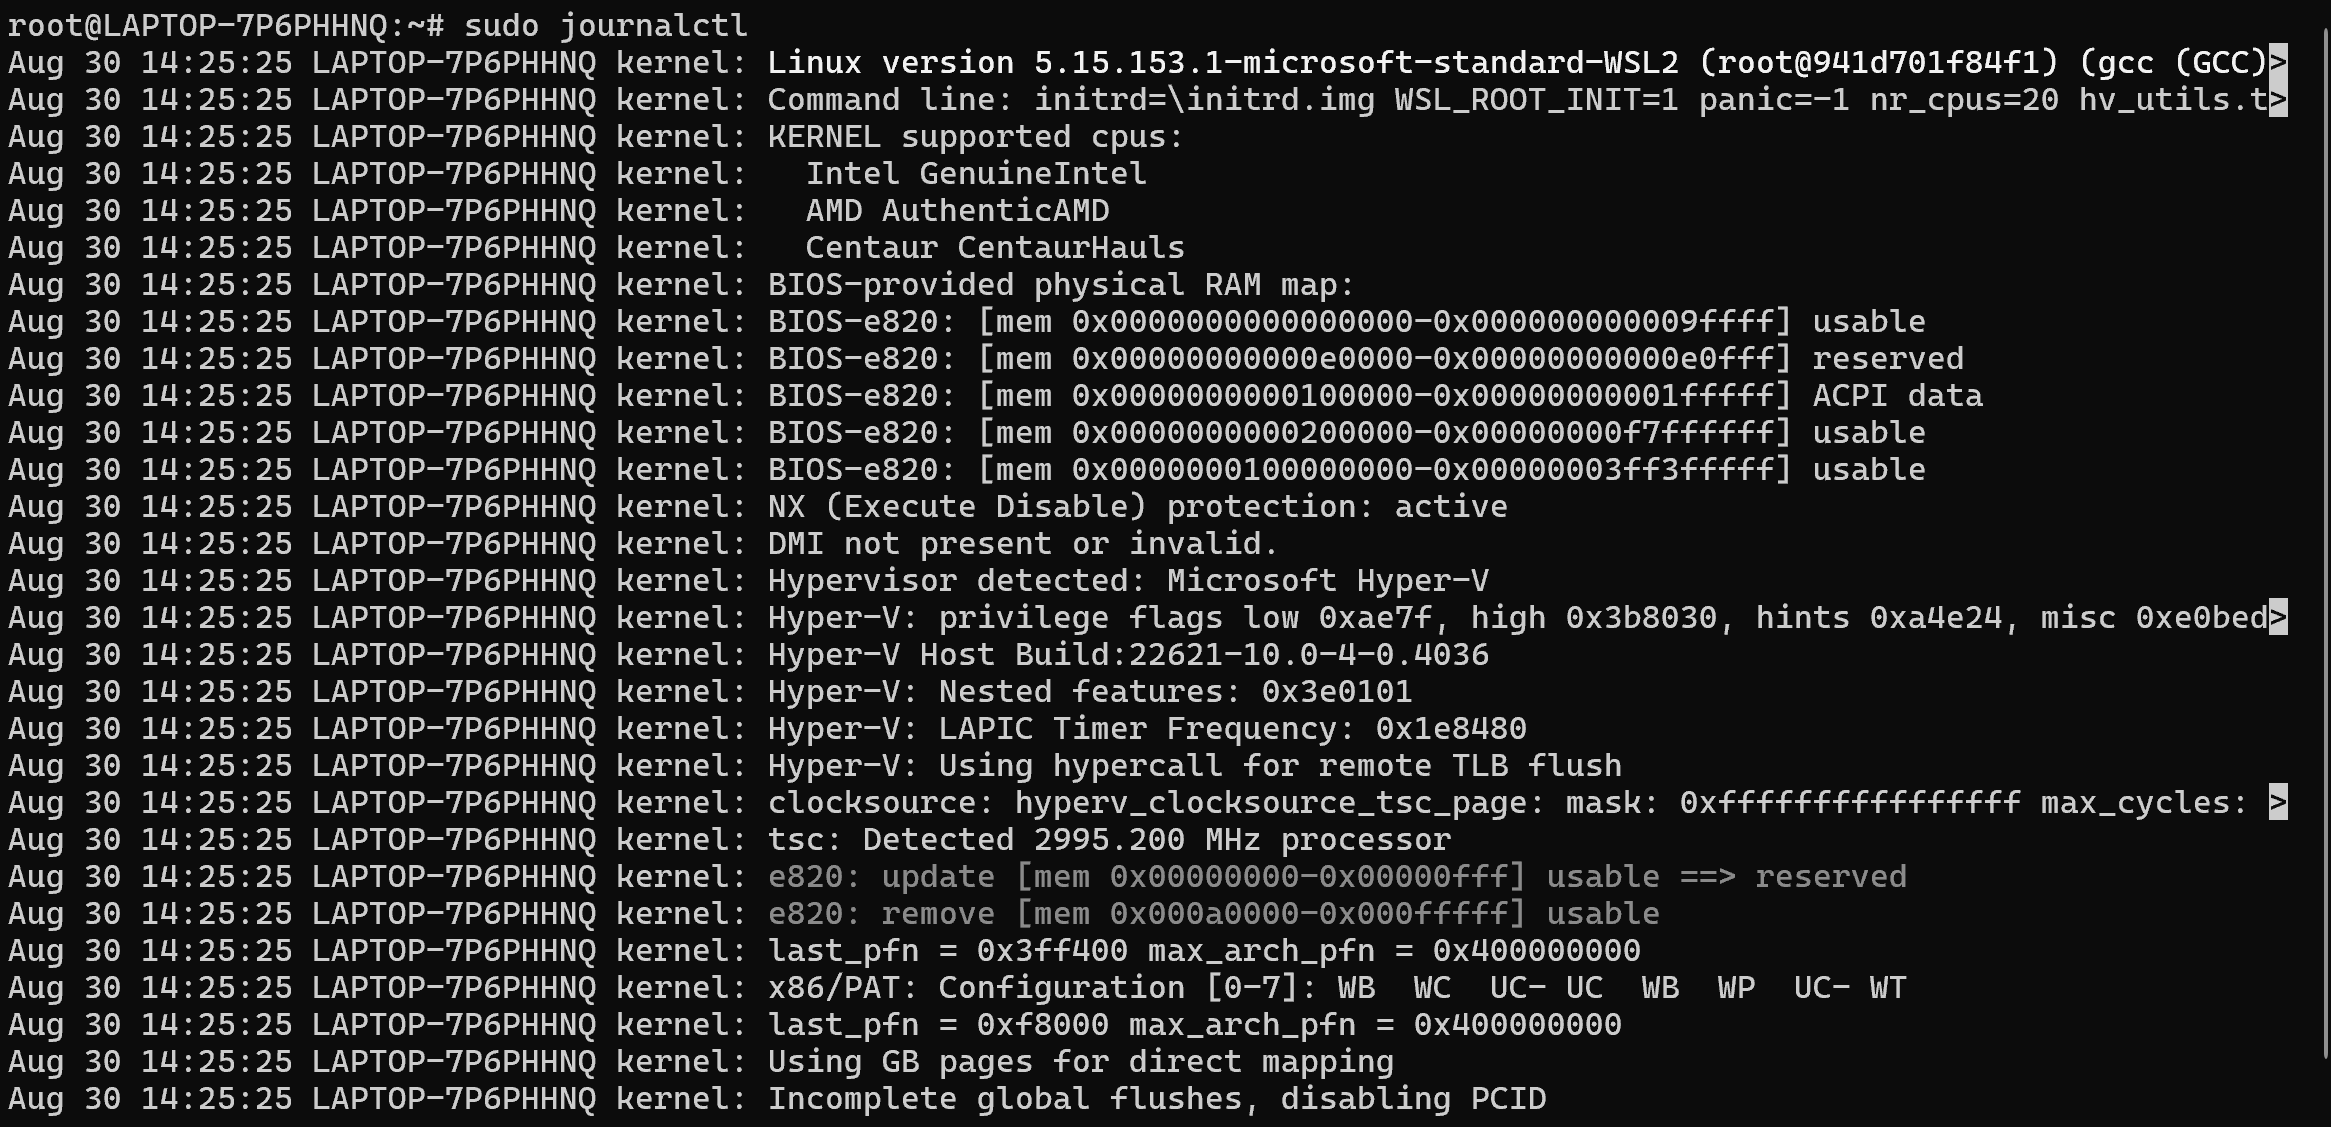
\includegraphics[width=\textwidth]{111} % 替换为您的第一张图片文件名
        \caption{效果}
        \label{fig:left}
    \end{subfigure}
    \hfill
    \begin{subfigure}[b]{0.48\textwidth}
        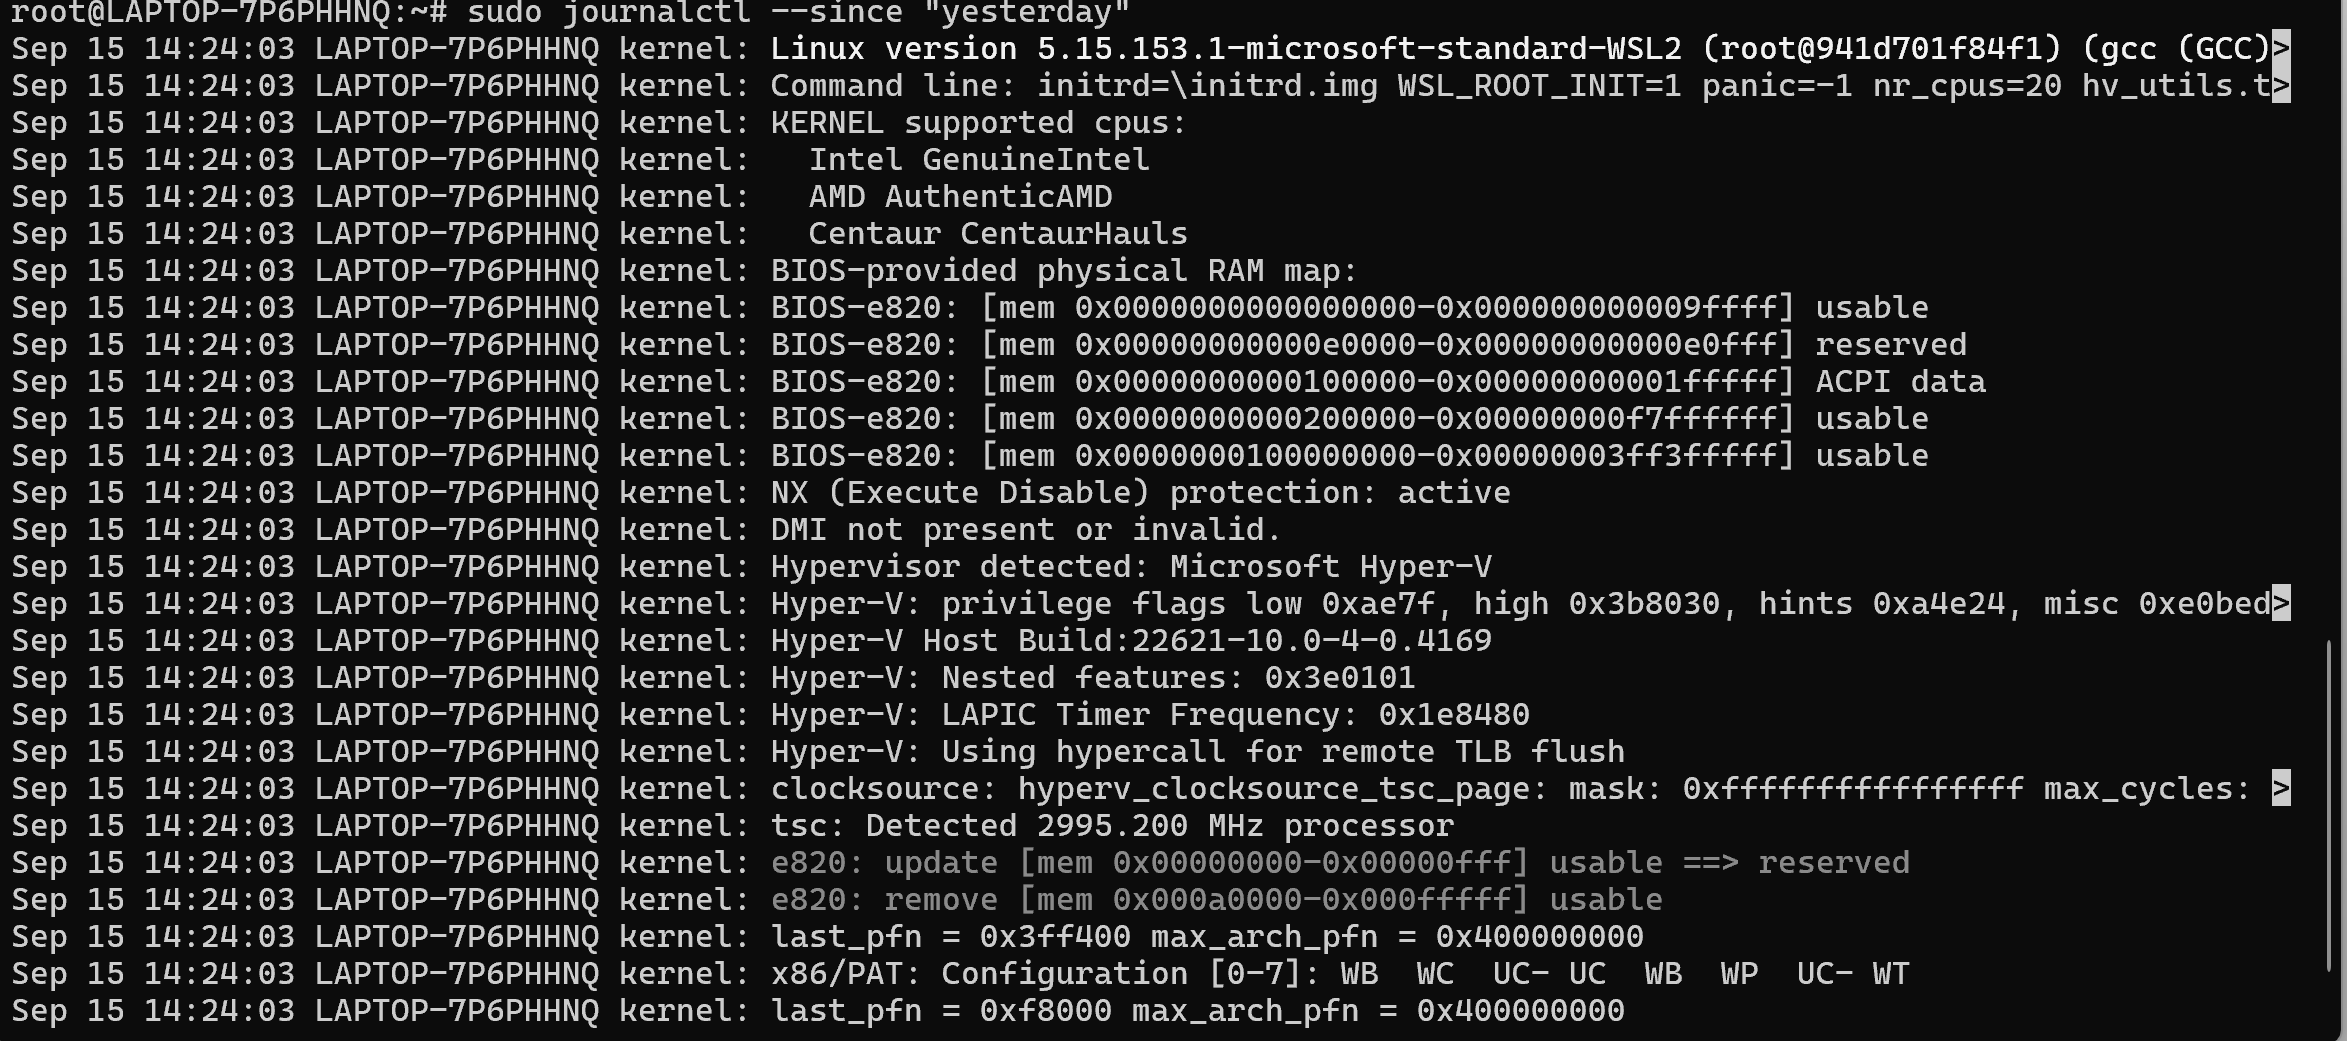
\includegraphics[width=\textwidth]{112} % 替换为您的第二张图片文件名
        \caption{效果}
        \label{fig:right}
    \end{subfigure}
    \caption{效果展示}
    \label{fig:side_by_side}
\end{figure}

 \begin{figure}[H]
    \centering
    \begin{subfigure}[b]{0.48\textwidth}
        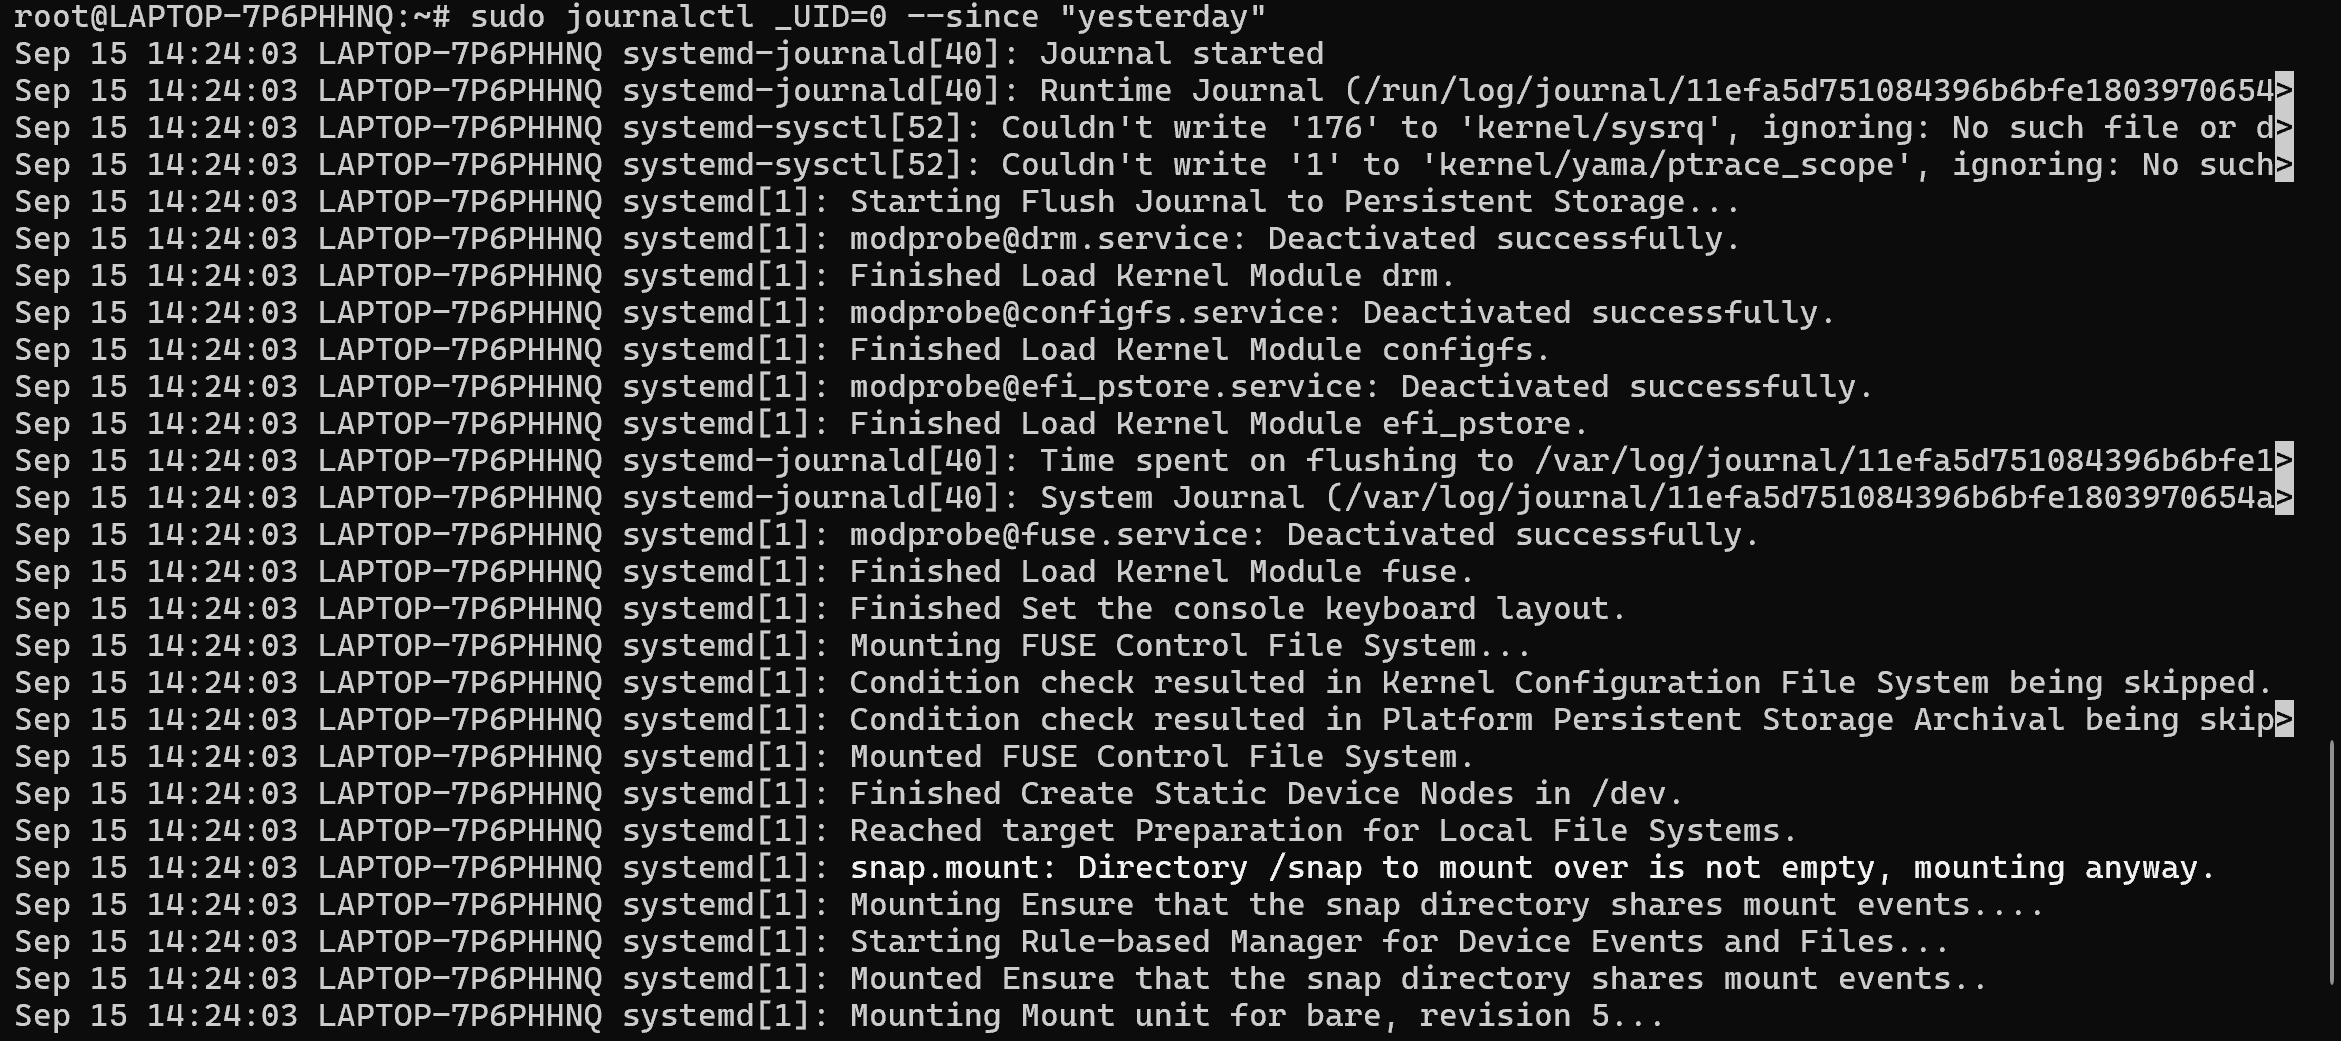
\includegraphics[width=\textwidth]{113} % 替换为您的第一张图片文件名
        \caption{效果}
        \label{fig:left}
    \end{subfigure}
    \hfill
    \begin{subfigure}[b]{0.48\textwidth}
        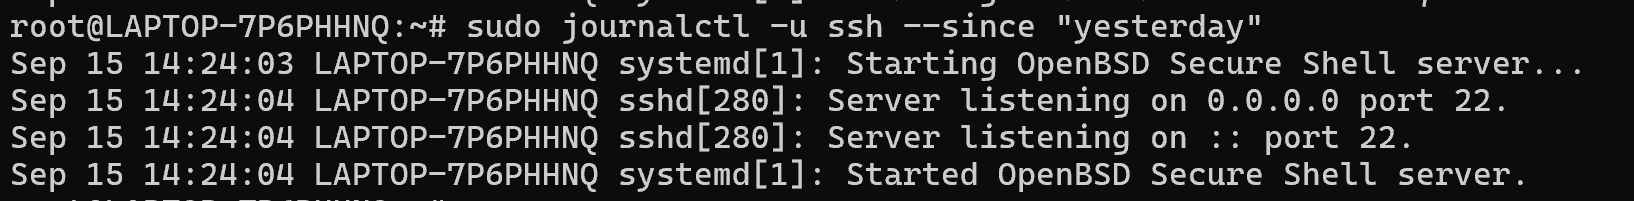
\includegraphics[width=\textwidth]{114} % 替换为您的第二张图片文件名
        \caption{效果}
        \label{fig:right}
    \end{subfigure}
    \caption{效果展示}
    \label{fig:side_by_side}
\end{figure}
  \end{itemize}
\end{enumerate}

%1.9LaTex=========================================================================%
%1.8LaTex=========================================================================%
\subsubsection{安装 shellcheck 并尝试检查以下脚本。}

\begin{enumerate}
  \item 获在编辑器中安装 linter 插件,以便自动获取警告。
  \begin{itemize}
  \item 命令展示
  \begin{verbatim}
安装 ShellCheck
sudo apt-get update
sudo apt-get install shellcheck

检查脚本



修复后的脚本
#!/bin/bash
## Example: a typical script with several problems
shopt -s nullglob  # This handles the case of no .m3u files gracefully
for f in *.m3u; do
  if grep -qi 'hq.*mp3' "$f"; then
    echo "Playlist $f contains a HQ file in mp3 format"
  fi
done


  \end{verbatim}
\item 效果展示
 \begin{figure}[H]
    \centering
    \begin{subfigure}[b]{0.48\textwidth}
        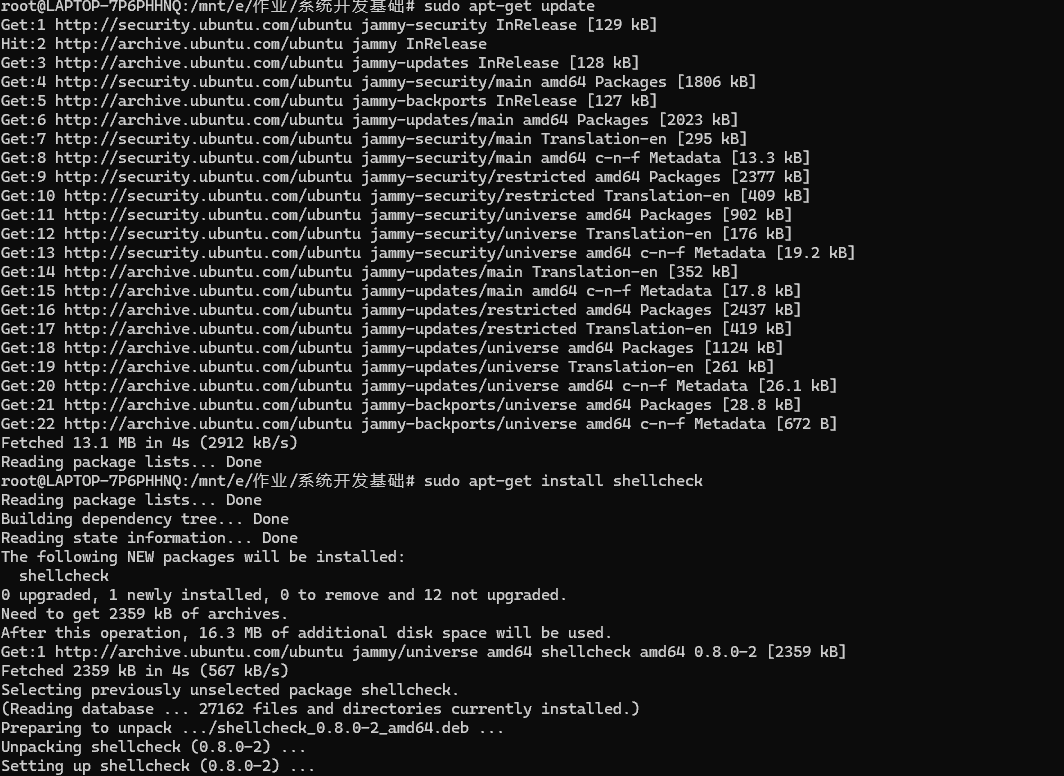
\includegraphics[width=\textwidth]{121} % 替换为您的第一张图片文件名
        \caption{效果}
        \label{fig:left}
    \end{subfigure}
    \hfill
    \begin{subfigure}[b]{0.48\textwidth}
        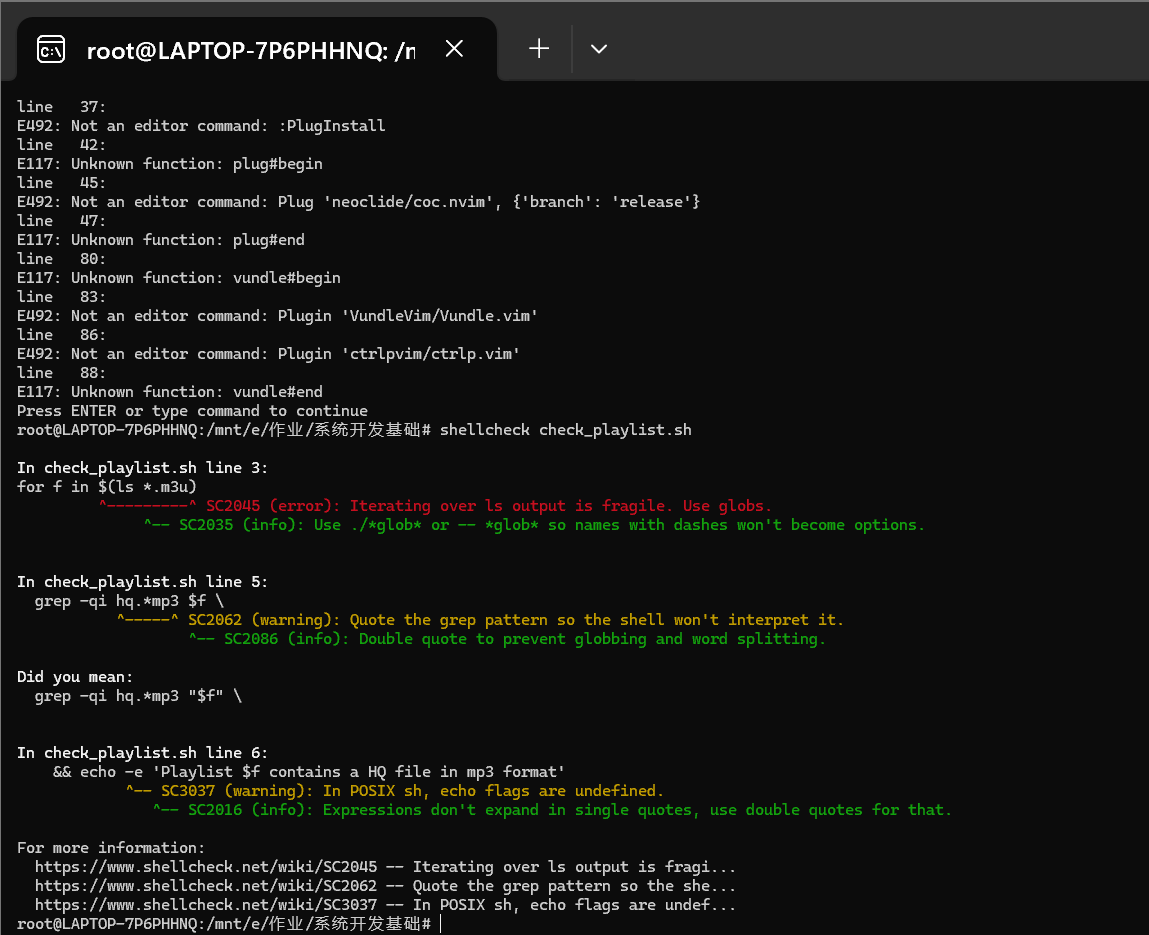
\includegraphics[width=\textwidth]{122} % 替换为您的第二张图片文件名
        \caption{效果}
        \label{fig:right}
    \end{subfigure}
    \caption{效果展示}
    \label{fig:side_by_side}
\end{figure}
  \end{itemize}
\end{enumerate}

%1.9LaTex=========================================================================%
%1.8LaTex=========================================================================%
\subsubsection{查看占用进程的pid}

\begin{enumerate}
  \item 侦听的端口已被另一个进程占用,找到该进程 pid 并通过运行 终止它。
  \begin{itemize}
  \item 命令展示
  \begin{verbatim}

 Linux
python3 -m http.server 8000
lsof -i :8000 | grep LISTEN
kill 12345


Windows
python -m http.server 8000
netstat -aon | findstr :8000
taskkill /PID 12345 /F

  \end{verbatim}
\item 效果展示
 \begin{figure}[H]
    \centering
    \begin{subfigure}[b]{0.48\textwidth}
        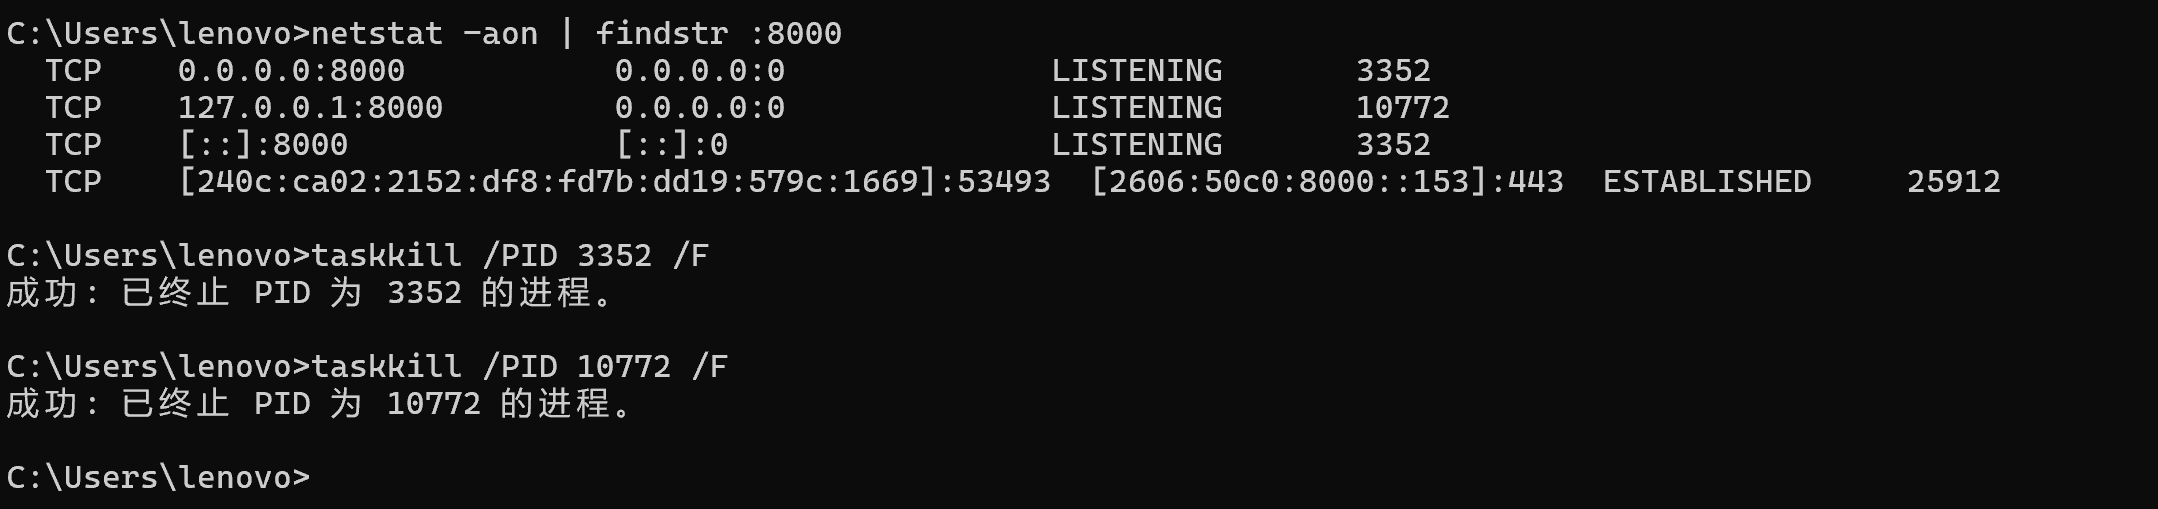
\includegraphics[width=\textwidth]{131} % 替换为您的第一张图片文件名
        \caption{效果}
        \label{fig:left}
    \end{subfigure}
    \hfill
    \begin{subfigure}[b]{0.48\textwidth}
        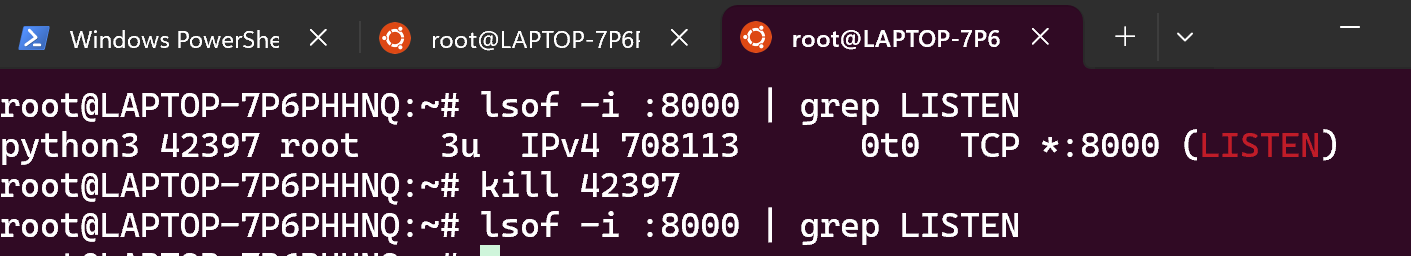
\includegraphics[width=\textwidth]{132} % 替换为您的第二张图片文件名
        \caption{效果}
        \label{fig:right}
    \end{subfigure}
    \caption{效果展示}
    \label{fig:side_by_side}
\end{figure}
  \end{itemize}
\end{enumerate}

%1.9LaTex=========================================================================%


%1.9LaTex=========================================================================%
\subsubsection{运行并使用 可视化 CPU 消耗。}

\begin{enumerate}
  \item 运行并使用 可视化 CPU 消耗
  \begin{itemize}
  \item 命令展示
  \begin{verbatim}
安装 stress 工具
sudo apt-get update
sudo apt-get install stress
stress -c 3
taskset --cpu-list 0,2 stress -c 3

查看 CPU 使用情况
sudo apt-get install htop
htop
创建和使用 cgroups
sudo apt-get install cgroup-tools
sudo cgcreate -g cpu,memory:/mygroup
echo 50000 | sudo tee /sys/fs/cgroup/cpu/mygroup/cpu.cfs_quota_us
echo 100000 | sudo tee /sys/fs/cgroup/cpu/mygroup/cpu.cfs_period_us
echo 100M | sudo tee /sys/fs/cgroup/memory/mygroup/memory.limit_in_bytes
sudo cgexec -g cpu,memory:/mygroup stress -c 3 -m 1
使用 cgroups 查看和调整资源限制
cat /sys/fs/cgroup/cpu/mygroup/cpu.cfs_quota_us
cat /sys/fs/cgroup/memory/mygroup/memory.limit_in_bytes






  \end{verbatim}
\item 效果展示
 \item 效果展示
  \begin{figure}[H]
    \centering
    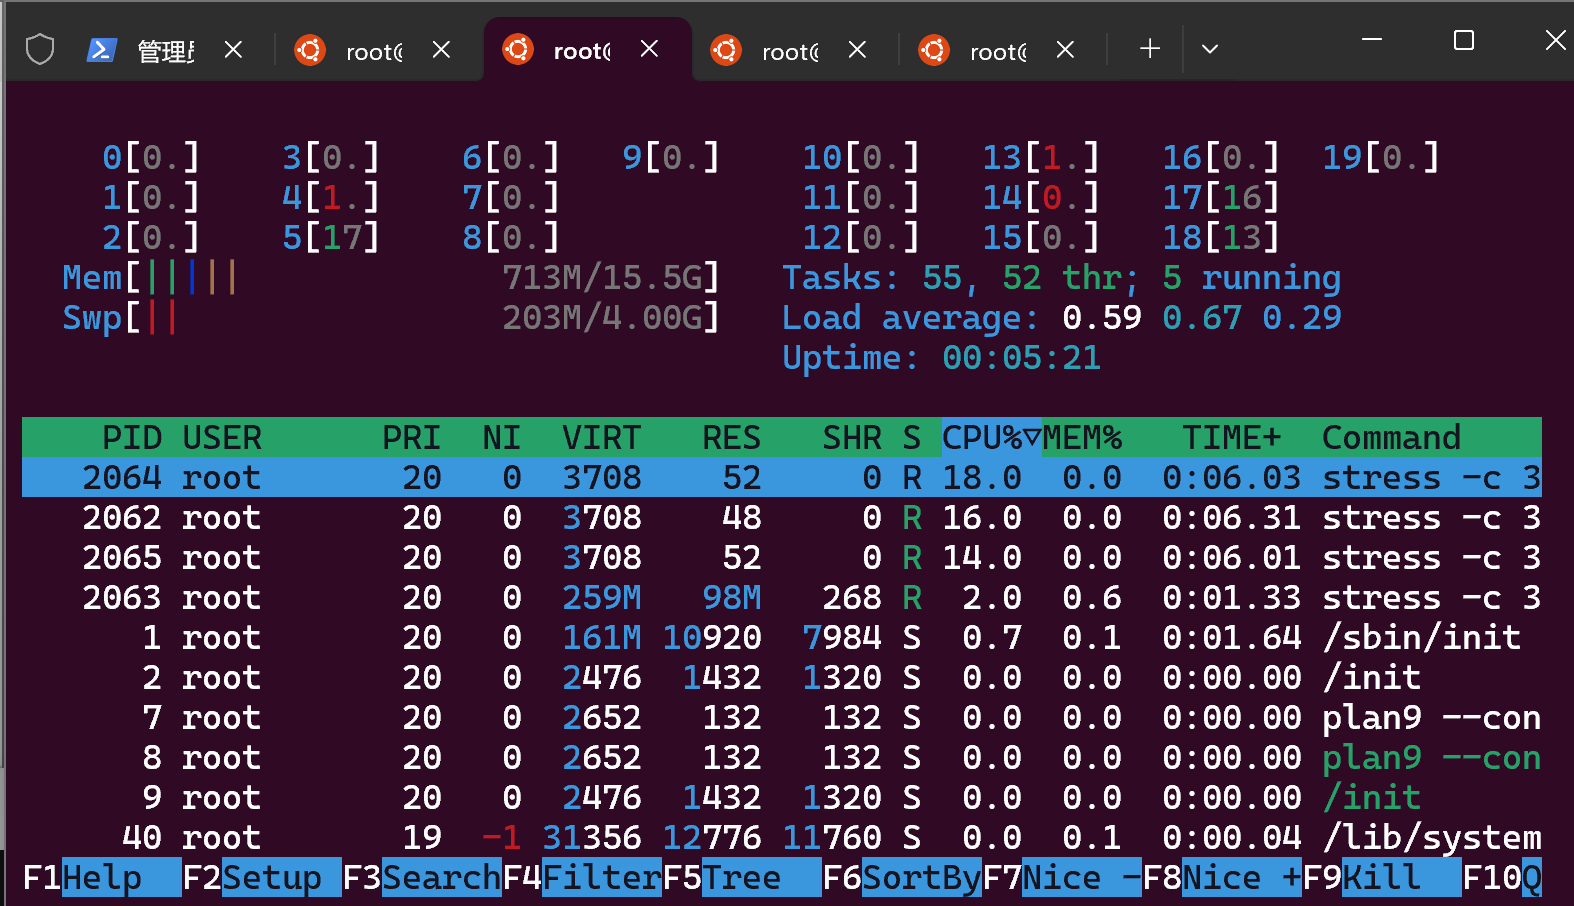
\includegraphics[width=\textwidth]{142} % 替换为您的图片文件名
    \caption{列表效果展示}
  \end{figure}
  \end{itemize}
\end{enumerate}


%1.2LaTex=========================================================================%
\subsubsection{执行 HTTP 请求并获取有关您的公有 IP 的信息。}

\begin{enumerate}
  \item 打开 Wireshark 并尝试嗅探发送和接收的请求和回复数据包。
  \begin{itemize}
  \item 命令展示
  \begin{verbatim}
sudo apt update
sudo apt install wireshark
sudo dnf install wireshark
sudo usermod -aG wireshark $USER

curl --version

sudo apt update
sudo apt install httpie

http
curl ipinfo.io

  \end{verbatim}
\item 效果展示
 \begin{figure}[H]
    \centering
    \begin{subfigure}[t]{0.32\textwidth}
        \centering
        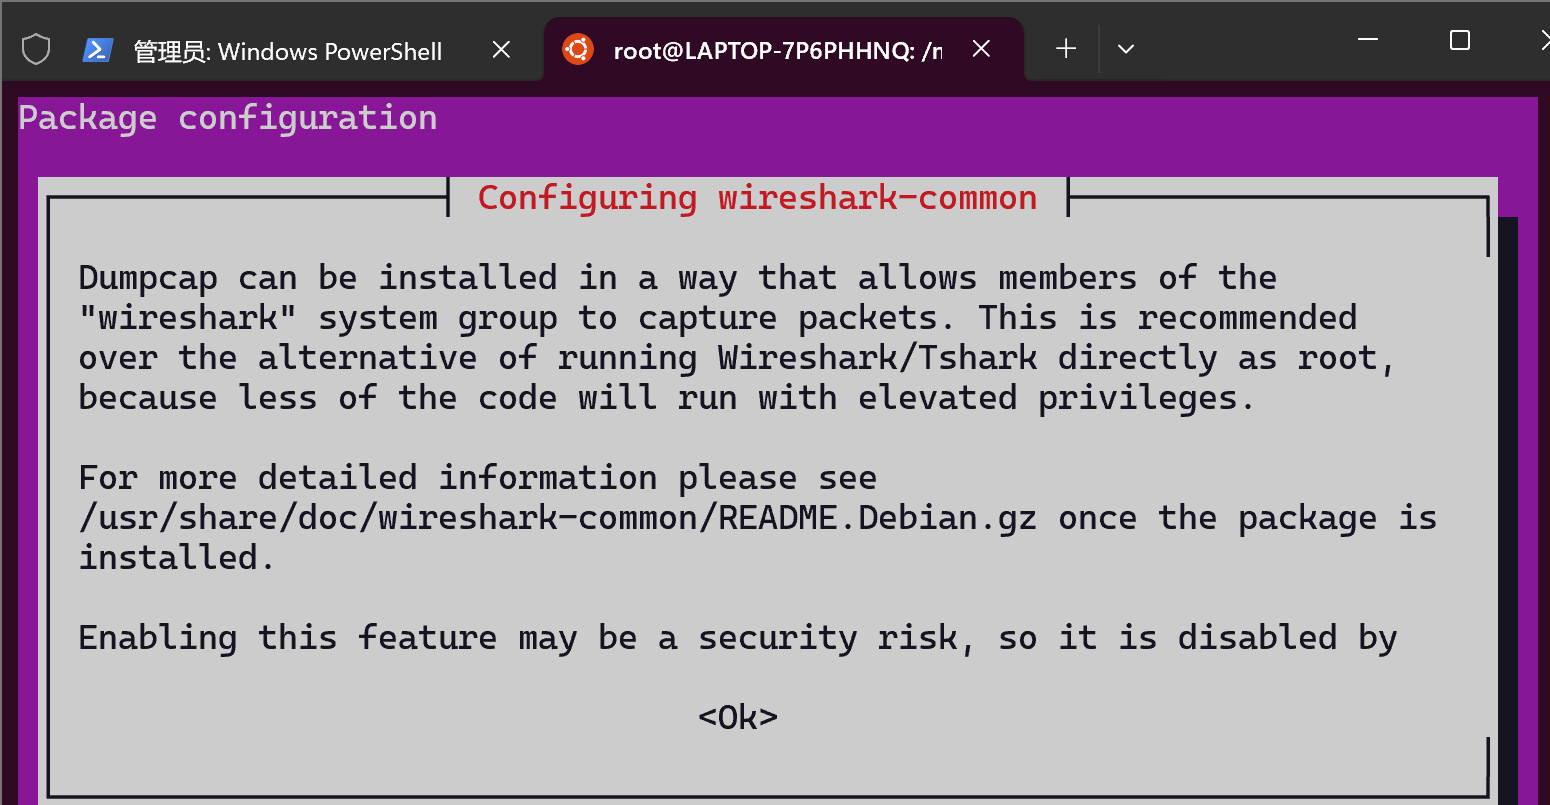
\includegraphics[width=\textwidth]{151} % 替换为您的第一张图片文件名
        \caption{展示}
    \end{subfigure}%
    \hfill
    \begin{subfigure}[t]{0.32\textwidth}
        \centering
        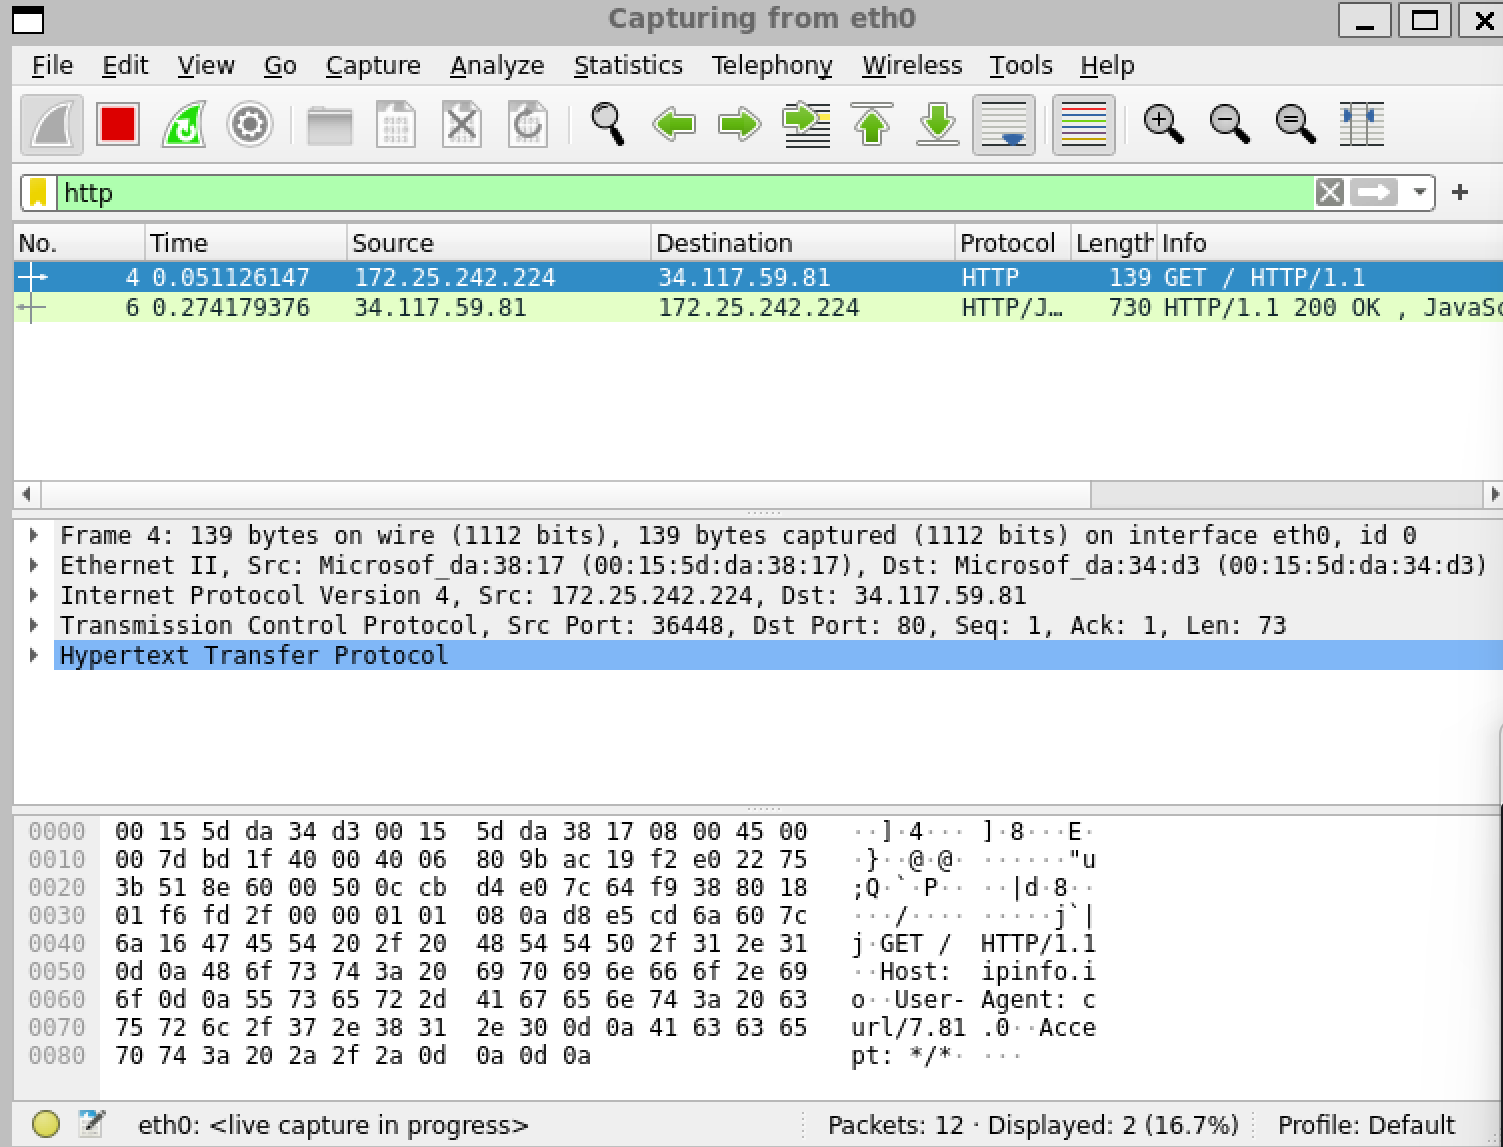
\includegraphics[width=\textwidth]{152} % 替换为您的第二张图片文件名
        \caption{展示}
    \end{subfigure}%
    \hfill
    \begin{subfigure}[t]{0.32\textwidth}
        \centering
        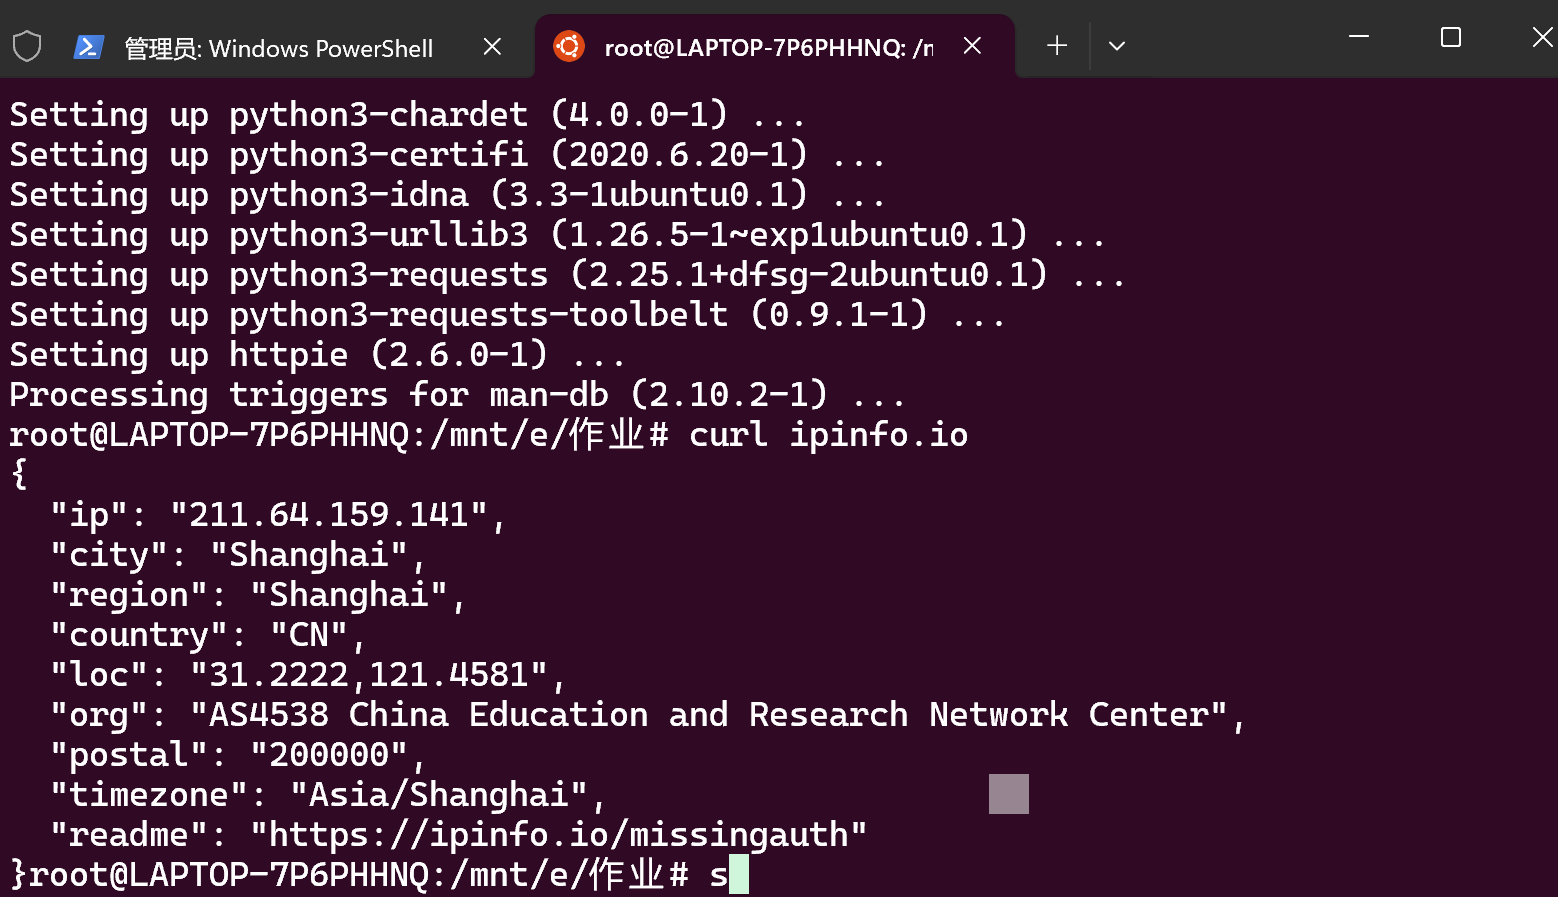
\includegraphics[width=\textwidth]{153} % 替换为您的第三张图片文件名
        \caption{展示}
    \end{subfigure}
    \caption{效果展示}
\end{figure}

  \end{itemize}
\end{enumerate}

%1.3LaTex=========================================================================%
\subsubsection{使用 GDB 调试 C/C++ 程序}

\begin{enumerate}
  \item 使用一个简单的程序来计算数组的平均值,但程序中存在一个错误。使用 GDB 来调试并找出问题所在。
  \begin{itemize}
  \item 命令展示
  \begin{verbatim}
c程序
#include <stdio.h>

float calculate_average(int *arr, int size) {
    int sum = 0;
    for (int i = 0; i <= size; i++) {  // 注意:这里有一个错误,应该是 i < size
        sum += arr[i];
    }
    return (float)sum / size;
}

int main() {
    int numbers[] = {1, 2, 3, 4, 5};
    int size = sizeof(numbers) / sizeof(numbers[0]);
    float average = calculate_average(numbers, size);
    printf("Average: %f\n", average);
    return 0;
}

gcc -g -o my_program my_program.c
gdb ./my_program
(gdb) break main
(gdb) run
(gdb) print my_variable

  \end{verbatim}\item 效果展示
\begin{figure}[H]
    \centering
    \begin{subfigure}[b]{0.48\textwidth}
        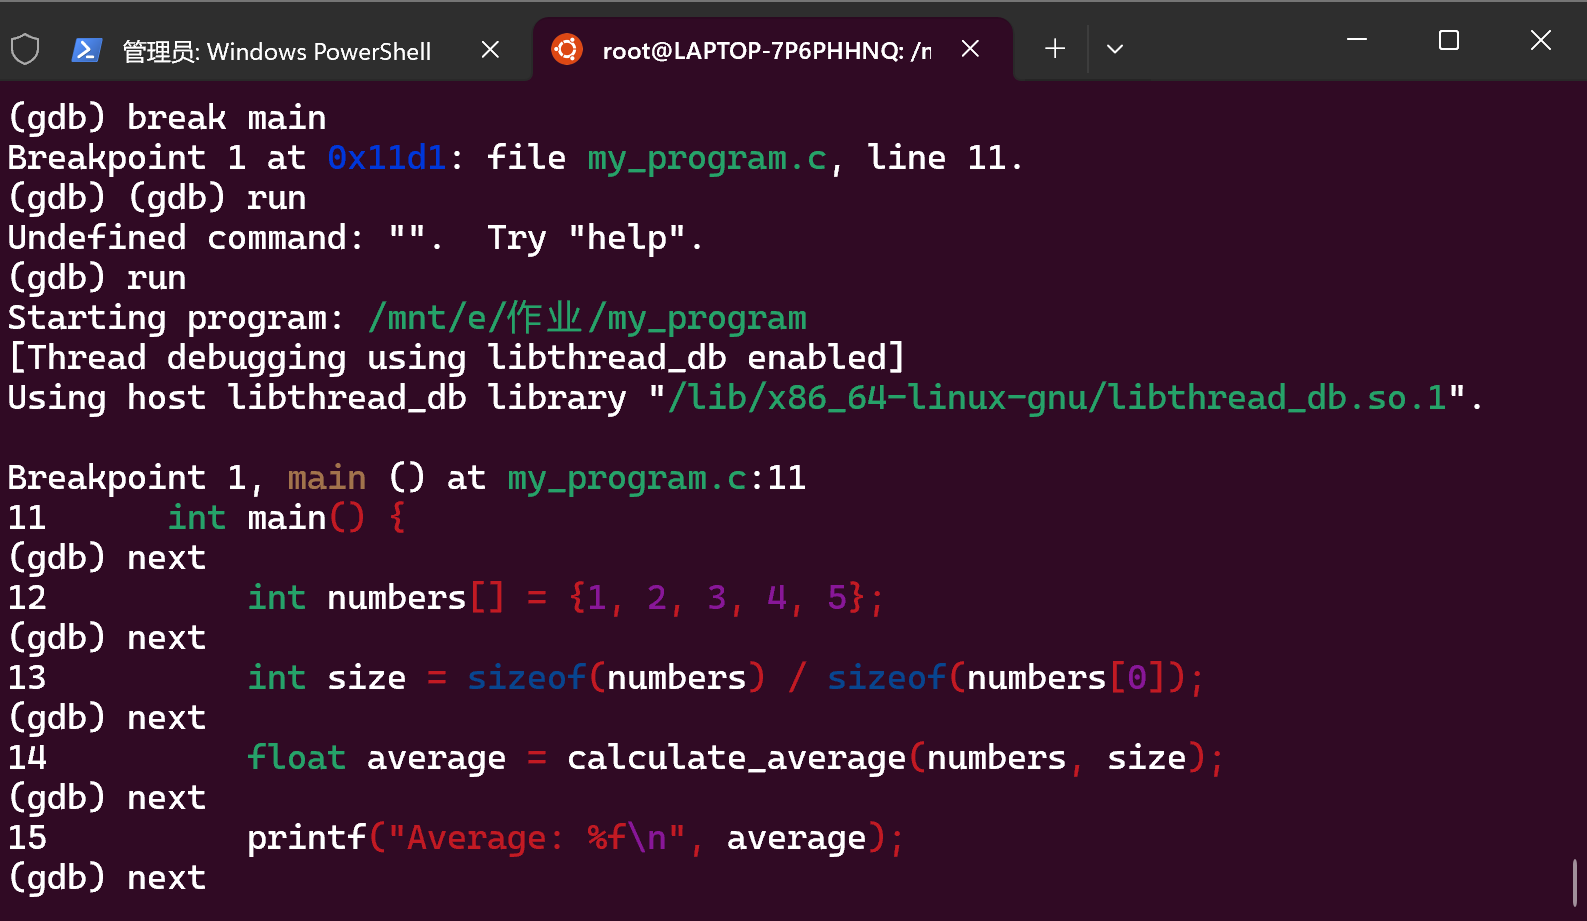
\includegraphics[width=\textwidth]{161} % 替换为您的第一张图片文件名
        \caption{效果}
        \label{fig:left}
    \end{subfigure}
    \hfill
    \begin{subfigure}[b]{0.48\textwidth}
        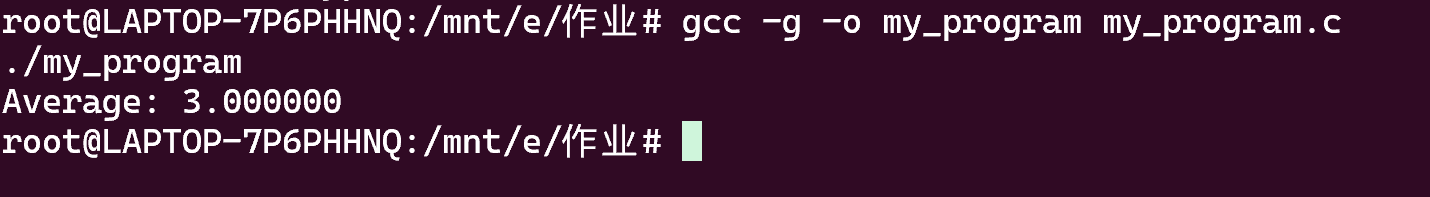
\includegraphics[width=\textwidth]{162} % 替换为您的第二张图片文件名
        \caption{修改之后}
        \label{fig:right}
    \end{subfigure}
    \caption{效果展示}
    \label{fig:side_by_side}
\end{figure}

  \end{itemize}
\end{enumerate}
%1.4LaTex=========================================================================%
\subsubsection{使用 strace 跟踪系统调用}

\begin{enumerate}
  \item 使用 strace 跟踪和分析一个简单 C 程序的系统调用。
  \begin{itemize}
  \item 命令展示
  \begin{verbatim}
c程序
#include <stdio.h>
#include <stdlib.h>

int main() {
    FILE *file = fopen("example.txt", "r");
    if (file == NULL) {
        perror("Failed to open file");
        return EXIT_FAILURE;
    }

    char buffer[256];
    while (fgets(buffer, sizeof(buffer), file)) {
        printf("%s", buffer);
    }

    fclose(file);
    return EXIT_SUCCESS;
}

echo "This is a test file.


gcc -o my_program my_program.c

strace -o strace_output.txt ./my_program
strace -e trace=open,close,read,write ./my_program


  \end{verbatim}
\item 效果展示
\begin{figure}[H]
    \centering
    \begin{subfigure}[t]{0.32\textwidth}
        \centering
        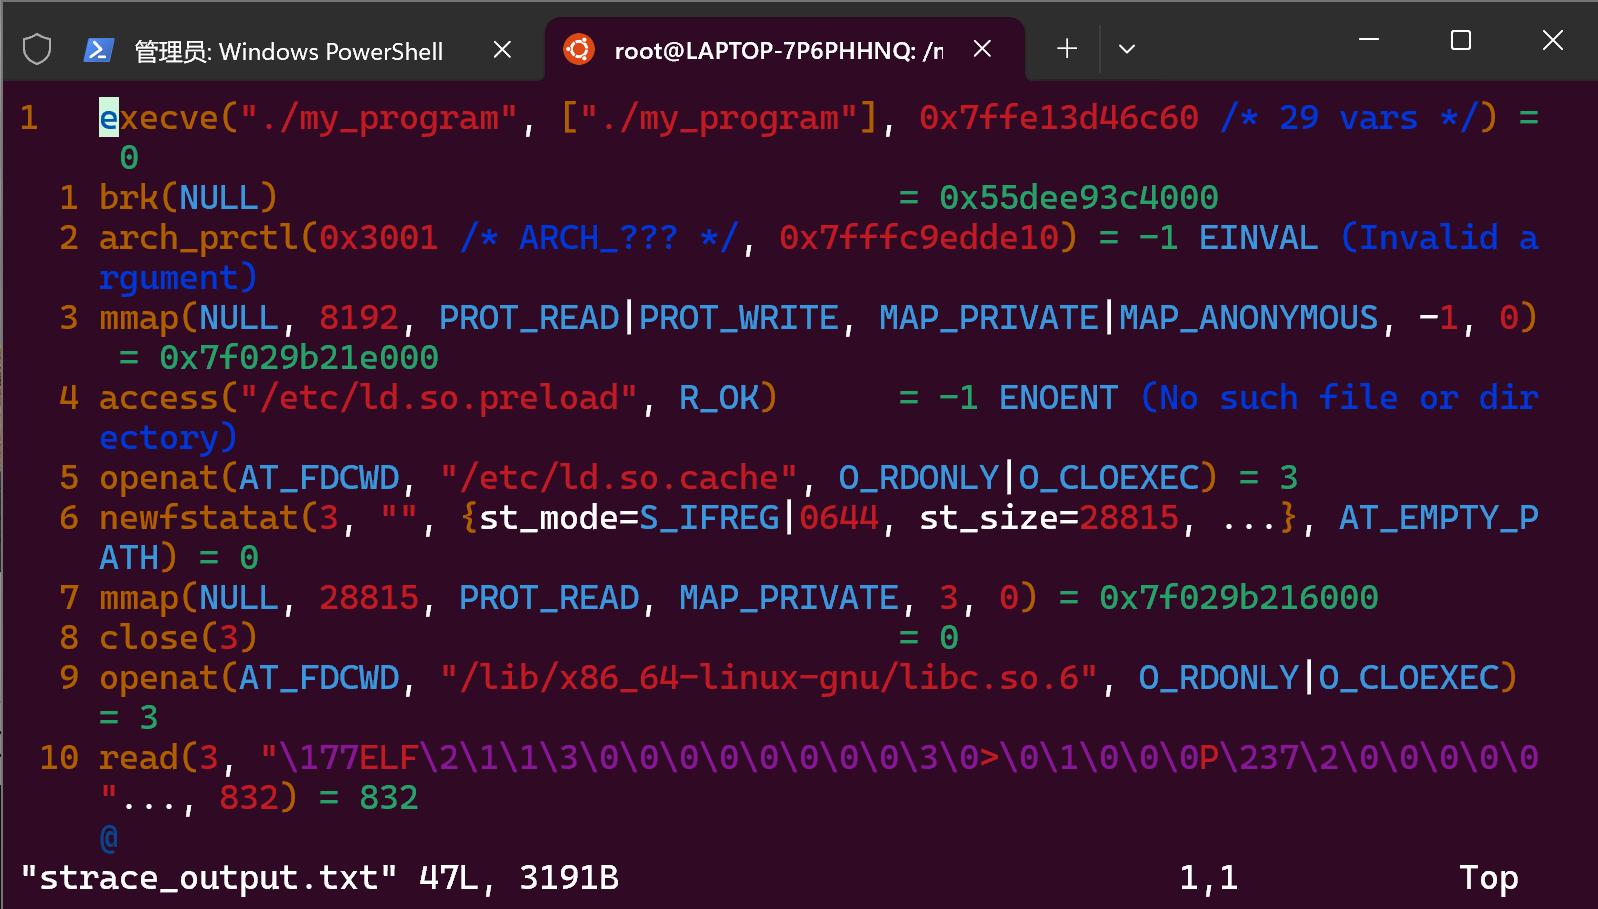
\includegraphics[width=\textwidth]{171} % 替换为您的第一张图片文件名
        \caption{展示}
    \end{subfigure}%
    \hfill
    \begin{subfigure}[t]{0.32\textwidth}
        \centering
        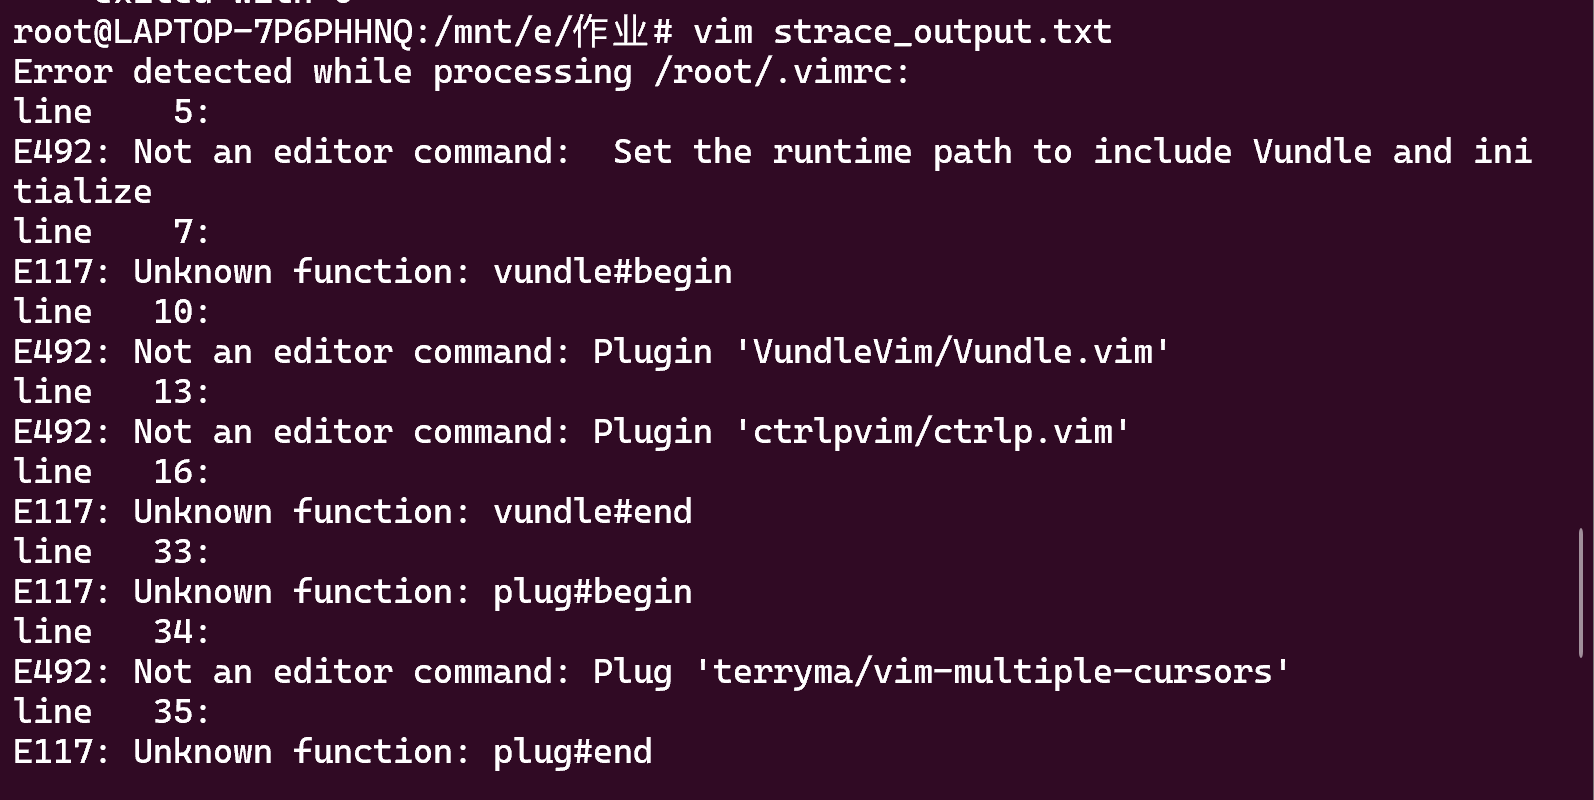
\includegraphics[width=\textwidth]{172} % 替换为您的第二张图片文件名
        \caption{展示}
    \end{subfigure}%
    \hfill
    \begin{subfigure}[t]{0.32\textwidth}
        \centering
        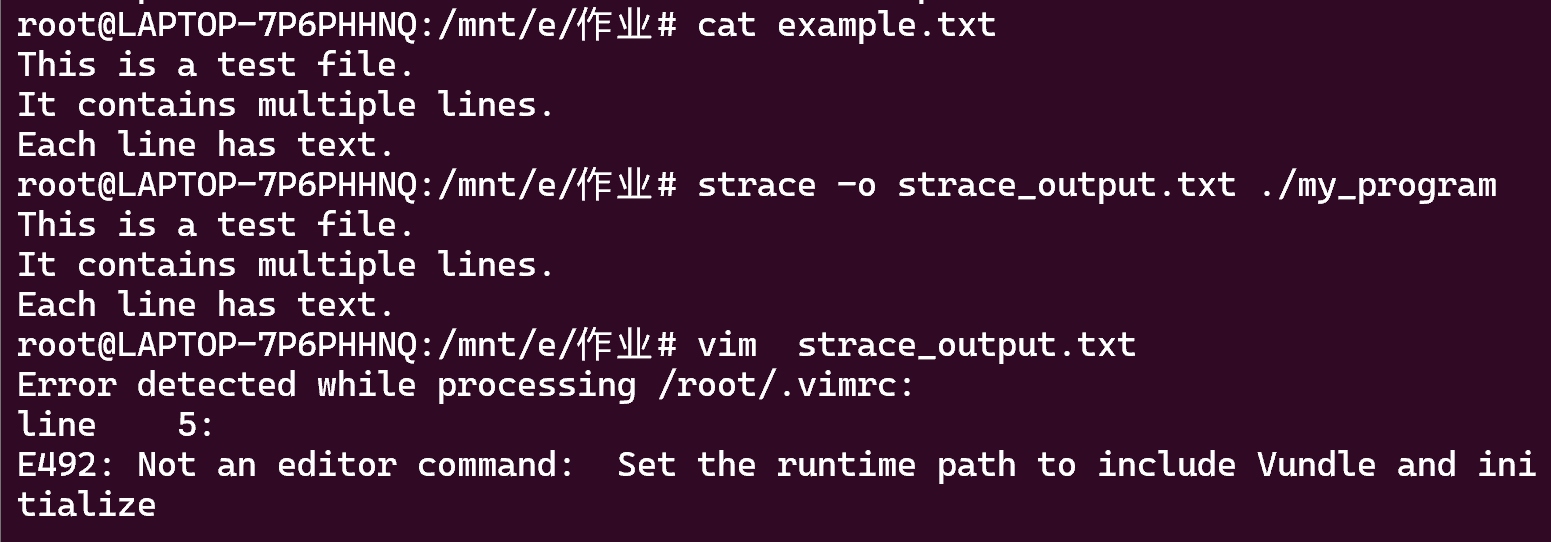
\includegraphics[width=\textwidth]{173} % 替换为您的第三张图片文件名
        \caption{展示}
    \end{subfigure}
    \caption{效果展示}
\end{figure}

  \end{itemize}
\end{enumerate}

%1.5LaTex=========================================================================%
\subsubsection{检测内存泄漏}

\begin{enumerate}
  \item 使用 Valgrind执行检测 C/C++ 程序内存泄漏和其他内存问题
  \begin{itemize}
  \item 命令展示
  \begin{verbatim}
sudo apt-get install valgrind

valgrind --leak-check=full ./my_program

c程序
#include <stdio.h>
#include <stdlib.h>

void create_memory_leak() {
    int *array = malloc(10 * sizeof(int)); // 分配内存但没有释放
    if (!array) {
        fprintf(stderr, "Memory allocation failed\n");
        return;
    }
    for (int i = 0; i < 10; i++) {
        array[i] = i * i;
    }
    // 忘记调用 free(array);
}

int main() {
    create_memory_leak();
    return 0;
}

gcc -g -o my_program my_program.c
修复内存泄漏
#include <stdio.h>
#include <stdlib.h>

void create_memory_leak() {
    int *array = malloc(10 * sizeof(int));
    if (!array) {
        fprintf(stderr, "Memory allocation failed\n");
        return;
    }
    for (int i = 0; i < 10; i++) {
        array[i] = i * i;
    }
    free(array); // 释放内存
}

int main() {
    create_memory_leak();
    return 0;
}

  \end{verbatim}
\item 效果展示
  \begin{figure}[H]
    \centering
    \begin{subfigure}[b]{0.48\textwidth}
        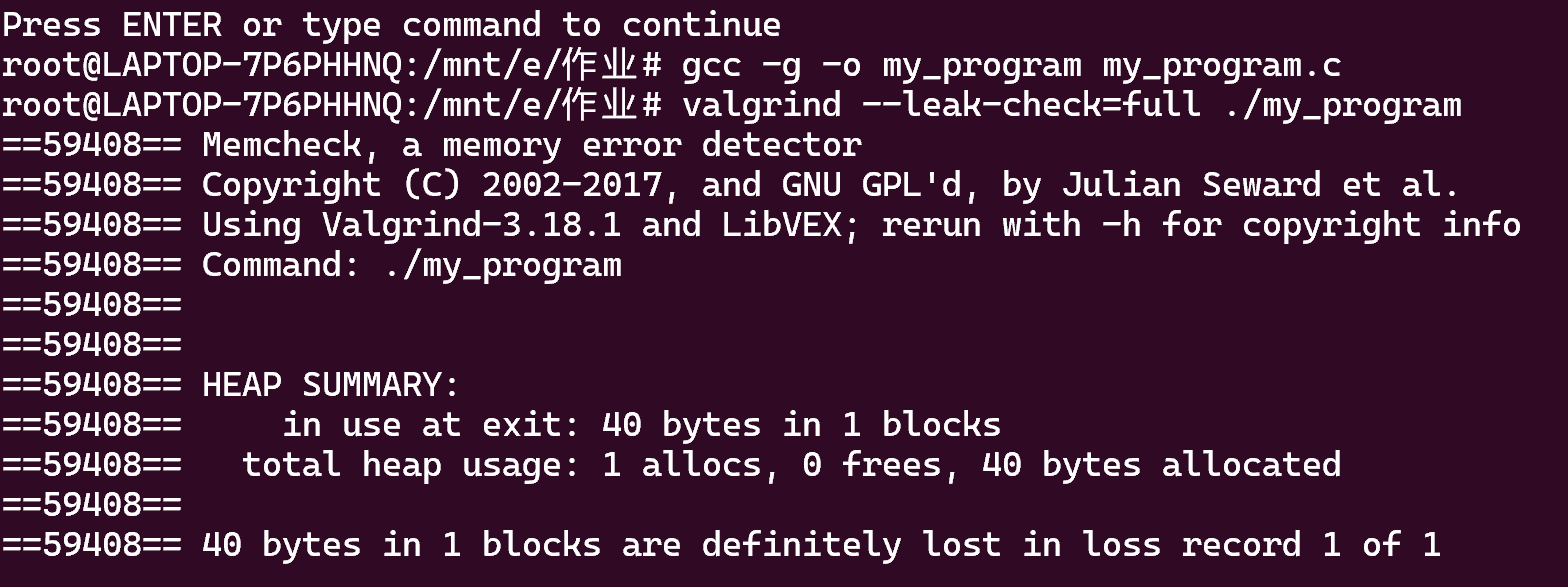
\includegraphics[width=\textwidth]{181} % 替换为您的第一张图片文件名
        \caption{效果}
        \label{fig:left}
    \end{subfigure}
    \hfill
    \begin{subfigure}[b]{0.48\textwidth}
        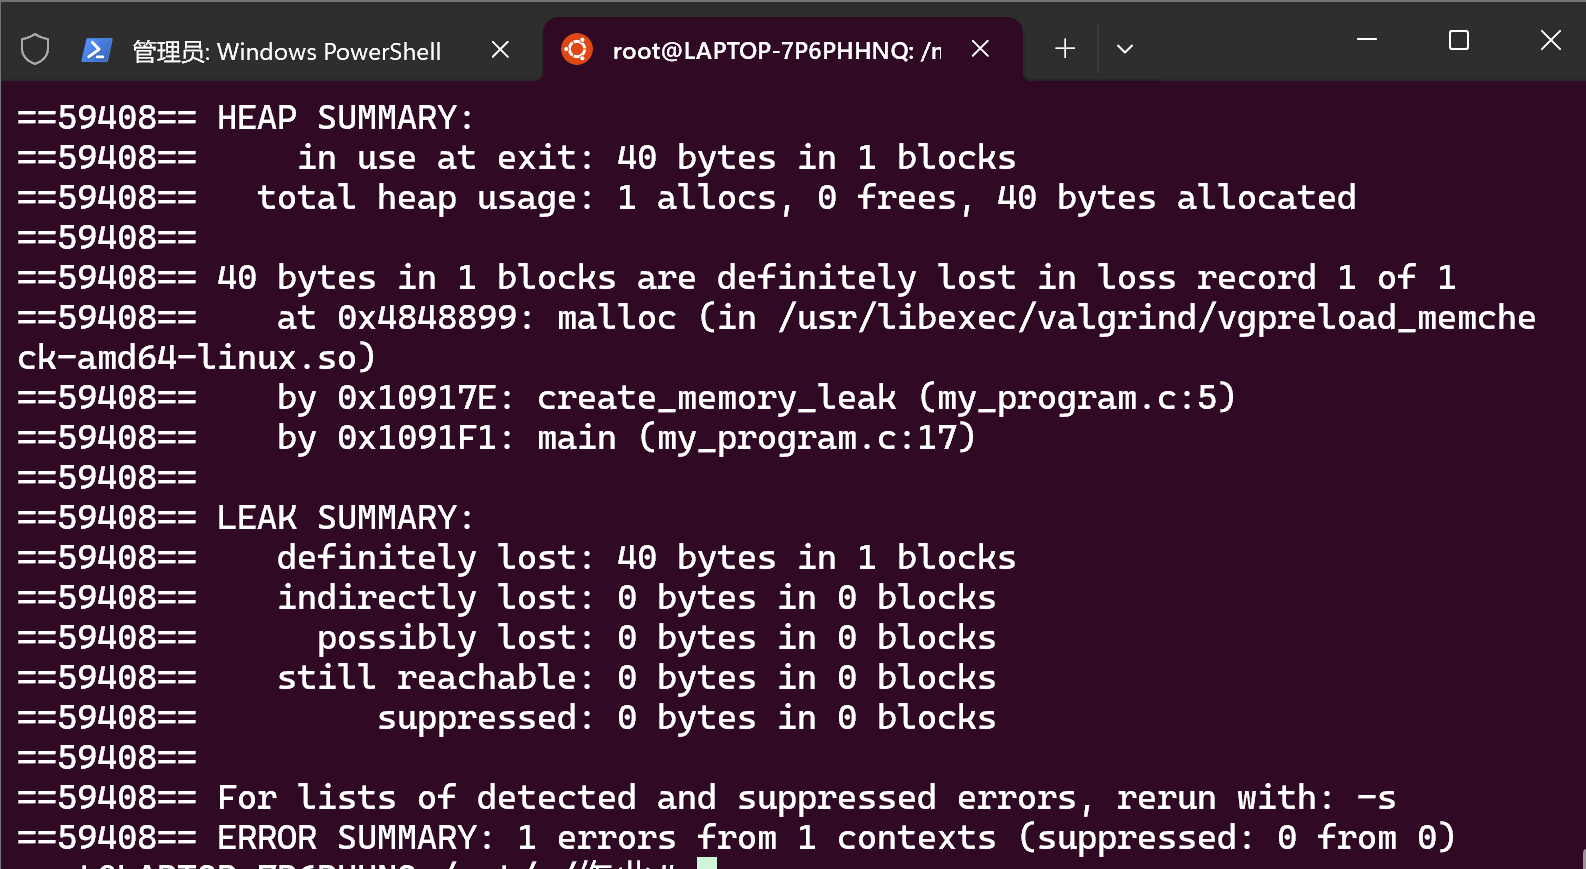
\includegraphics[width=\textwidth]{182} % 替换为您的第二张图片文件名
        \caption{效果}
        \label{fig:right}
    \end{subfigure}
    \caption{效果展示}
    \label{fig:side_by_side}
\end{figure}
  \end{itemize}
\end{enumerate}

%1.6LaTex=========================================================================%
\subsubsection{使用 perf 分析程序性能}

\begin{enumerate}
  \item 使用 perf 分析程序性能
  \begin{itemize}
  \item 命令展示
  \begin{verbatim}
c程序
#include <stdio.h>
#include <stdlib.h>

void compute_squares(int *array, int size) {
    for (int i = 0; i < size; i++) {
        array[i] = i * i;
    }
}

int main() {
    int size = 1000000; // 1 million elements
    int *array = malloc(size * sizeof(int));
    if (!array) {
        fprintf(stderr, "Memory allocation failed\n");
        return 1;
    }

    compute_squares(array, size);

    printf("Computation completed\n");
    free(array);
    return 0;
}
sudo apt-get update
sudo apt-get install linux-tools-common linux-tools-generic

gcc -O2 -o my_program my_program.c
perf record -g ./my_program
perf report


  \end{verbatim}
\item 效果展示
  \begin{figure}[H]
    \centering
    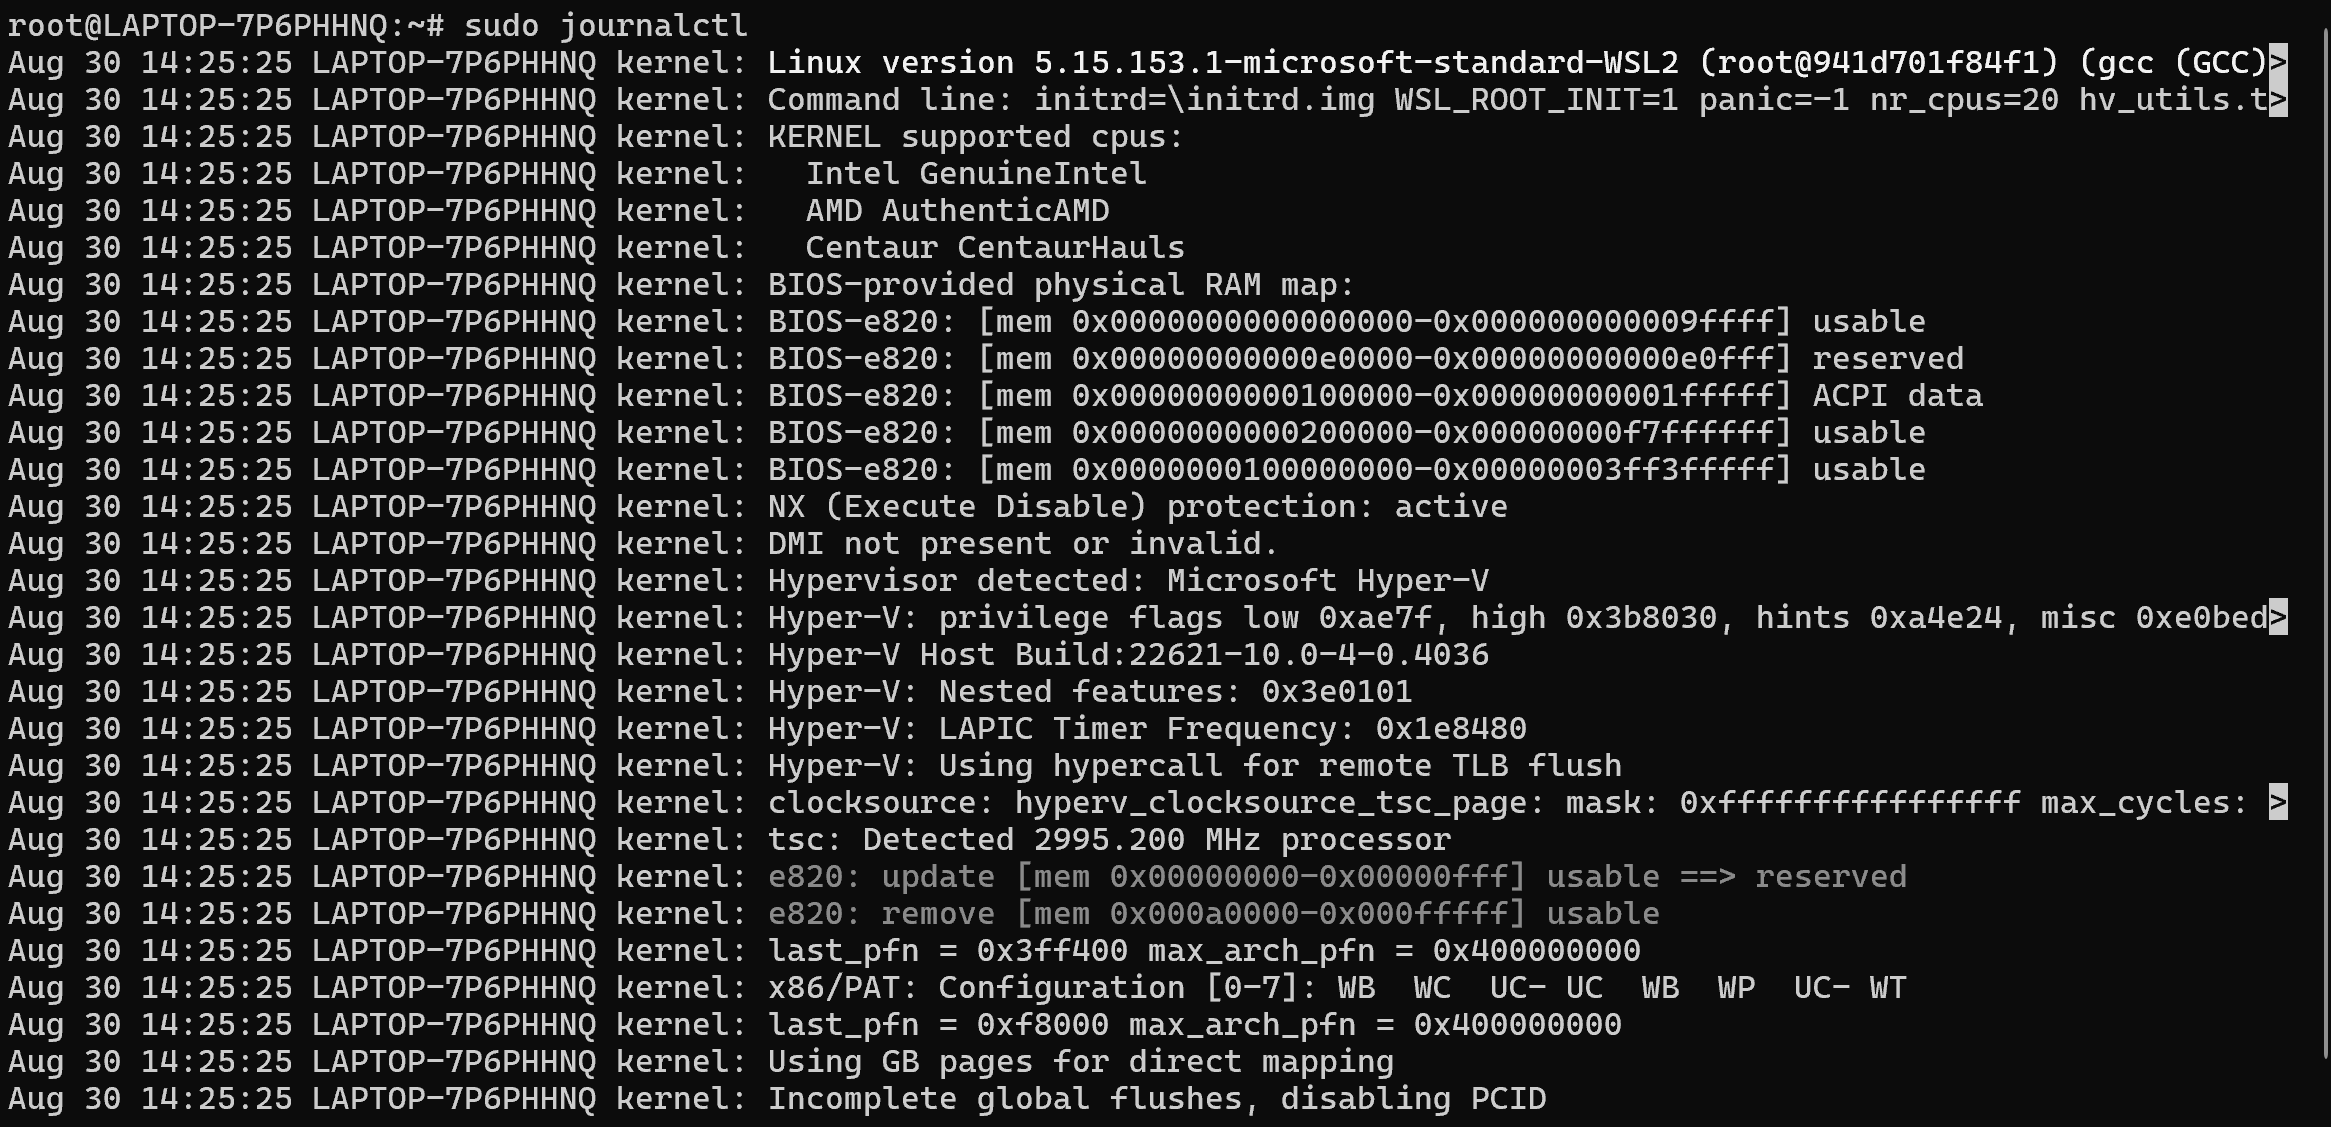
\includegraphics[width=\textwidth]{111} % 替换为您的图片文件名
    \caption{列表效果展示}
  \end{figure}
  \end{itemize}
\end{enumerate}

%1.7LaTex=========================================================================%


%1.8LaTex=========================================================================%


%1.9LaTex=========================================================================%


%1.10LaTex=========================================================================%

%1.11LaTex=========================================================================%



































































%1.2LaTex=========================================================================%
  \subsection{元编程演示实验}
  {\color{blue}元编程演示实验展示}











%2.1LaTex=========================================================================%
\subsubsection{make 重新构建}

\begin{enumerate}
  \item 在 Makefile 中实现一个 clean 目标,删除构建过程中生成的所有文件
  \begin{itemize}
  \item 命令展示
  \begin{verbatim}
list = [1, 2, 3, 'frist', 9.0]
ok = [99, 'I am ']
ok.extend(list)
print(list)
print(list[0])
print(list[1:3])
print(list[2:])
print(ok * 2)
print(list + ok)
print(ok)
print(ok.index('frist'))
print(ok.count('frist'))
print(ok.pop(2))
print(ok)
ok.reverse()
print(ok)

    
  \end{verbatim}

  \item 效果展示

\begin{figure}[H]
    \centering
    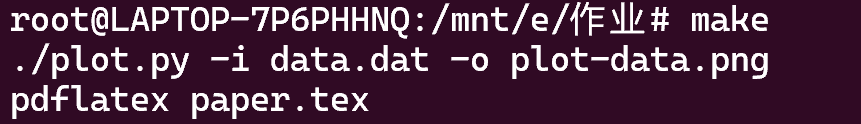
\includegraphics[width=\textwidth]{21} % 确保文件名正确
    
\end{figure}
\end{itemize}
\end{enumerate}
















%2.2LaTex=========================================================================%
\subsubsection{动态创建类和方法}

\begin{enumerate}
  \item 用元类(metaclass)来动态创建一个具有加法、减法和乘法功能的数学类
  \begin{itemize}
    \item 命令展示
    \begin{verbatim}
# 定义一个元类
class MathMeta(type):
    def __new__(cls, name, bases, attrs):
        # 动态添加方法
        def add(self, a, b):
            return a + b

        def subtract(self, a, b):
            return a - b

        def multiply(self, a, b):
            return a * b

        # 把新方法添加到类属性中
        attrs['add'] = add
        attrs['subtract'] = subtract
        attrs['multiply'] = multiply

        # 创建类
        return super().__new__(cls, name, bases, attrs)

# 使用元类创建一个新的数学类
class MathOperations(metaclass=MathMeta):
    pass

# 使用动态创建的类
math_op = MathOperations()

# 测试动态添加的方法
print("加法: 5 + 3 =", math_op.add(5, 3))          # 输出: 加法: 5 + 3 = 8
print("减法: 5 - 3 =", math_op.subtract(5, 3))      # 输出: 减法: 5 - 3 = 2
print("乘法: 5 * 3 =", math_op.multiply(5, 3))      # 输出: 乘法: 5 * 3 = 15
    \end{verbatim}

    \item 效果展示
    \begin{figure}[H]
      \centering
      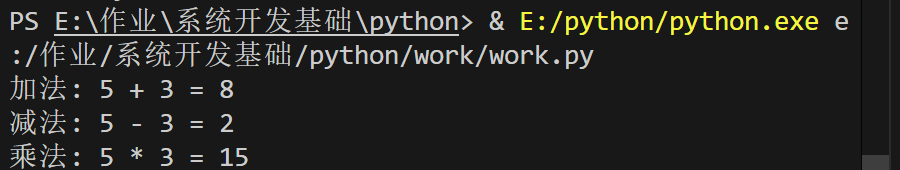
\includegraphics[width=\textwidth]{22} % 确保文件名正确
      \caption{效果展示}
    \end{figure}
  \end{itemize}
\end{enumerate}




















%2.3LaTex=========================================================================%
\subsubsection{动态属性添加}

\begin{enumerate}
  \item 创建一个类,它可以在运行时动态添加属性。
  \begin{itemize}
  \item 命令展示
  \begin{verbatim}
class DynamicAttributes:
    def __init__(self):
        self.existing_attribute = "I already exist!"

    def __setattr__(self, name, value):
        print(f"Setting attribute '{name}' to '{value}'")
        super().__setattr__(name, value)

# 创建实例
obj = DynamicAttributes()

# 添加动态属性
obj.new_attribute = "I am new!"
print(obj.existing_attribute)
print(obj.new_attribute)



    
  \end{verbatim}

  \item 效果展示
  \begin{figure}[H]
    \centering
    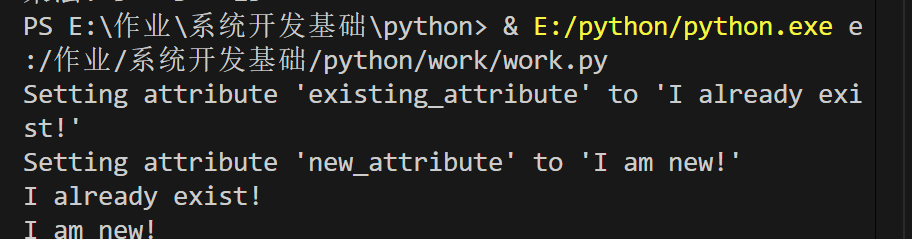
\includegraphics[width=\textwidth]{24} % 确保文件名正确
    \caption{效果展示}
  
  \end{figure}
\end{itemize}
\end{enumerate}
























%2.4LaTex=========================================================================%
\subsubsection{使用元类进行属性验证}

\begin{enumerate}
  \item 定义一个元类,用于在创建类时验证某些属性的类型。
  \begin{itemize}
  \item 命令展示
  \begin{verbatim}
 
class TypedMeta(type):
    def __new__(cls, name, bases, attrs):
        # 检查属性类型
        for attr_name, attr_value in attrs.items():
            if isinstance(attr_value, type):
                attrs[attr_name] = attr_value()
        
        return super().__new__(cls, name, bases, attrs)

class Person(metaclass=TypedMeta):
    name = str
    age = int

    def __init__(self):
        self.name = "John Doe"
        self.age = 30

# 使用示例
person = Person()
print(f"Name: {person.name}, Age: {person.age}")
# 输出: Name: John Doe, Age: 30


    
  \end{verbatim}

  \item 效果展示
  \begin{figure}[H]
    \centering
    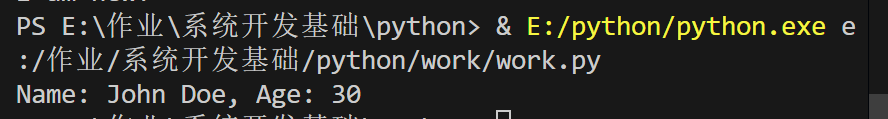
\includegraphics[width=\textwidth]{25} % 确保文件名正确
    \caption{效果展示}
  
  \end{figure}
\end{itemize}
\end{enumerate}

















%2.5LaTex=========================================================================%
\subsubsection{使用装饰器进行方法计时}

\begin{enumerate}
  \item 使用装饰器来记录方法调用的时间。
  \begin{itemize}
  \item 命令展示
  \begin{verbatim}
import time

def timing_decorator(func):
    def wrapper(*args, **kwargs):
        start_time = time.time()
        result = func(*args, **kwargs)
        end_time = time.time()
        print(f"Method {func.__name__} took {end_time - start_time:.4f} seconds to execute.")
        return result
    return wrapper

class MathOperations:
    @timing_decorator
    def add(self, a, b):
        time.sleep(1)  # 模拟耗时操作
        return a + b

# 使用示例
math_op = MathOperations()
result = math_op.add(5, 3)
print("Result:", result)  # 输出: Result: 8


    
  \end{verbatim}

  \item 效果展示
  \begin{figure}[H]
    \centering
    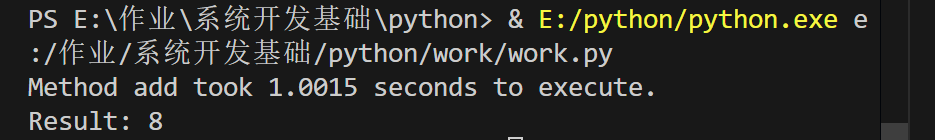
\includegraphics[width=\textwidth]{266} % 确保文件名正确
    \caption{效果展示}
  
  \end{figure}
\end{itemize}
\end{enumerate}





















%2.6LaTex=========================================================================%
\subsubsection{使用元类实现只读属性}

\begin{enumerate}
  \item 创建一个元类,该元类会将指定的属性设置为只读。即这些属性只能在对象创建时赋值,之后不能再次修改。
  \begin{itemize}
  \item 命令展示
  \begin{verbatim}
 class ReadOnlyMeta(type):
    def __new__(cls, name, bases, attrs):
        # 找到以 _readonly_ 开头的属性并将其设置为只读
        for attr_name, attr_value in attrs.items():
            if isinstance(attr_value, str) and attr_name.startswith('_readonly_'):
                # 创建新的属性,只能在初始化时赋值
                original_value = attr_value

                def getter(self, name=attr_name):
                    return getattr(self, "_" + name)

                # 创建一个设置器,抛出异常
                def setter(self, value, name=attr_name):
                    raise AttributeError(f"{name} 是只读属性,不能被修改。")

                # 将属性设置为只读
                attrs[attr_name] = property(getter, setter)
                attrs["_" + attr_name] = original_value

        return super().__new__(cls, name, bases, attrs)

class Person(metaclass=ReadOnlyMeta):
    _readonly_name = "John Doe"
    _readonly_age = 30

# 使用示例
person = Person()
print(person._readonly_name)  # 输出: John Doe
print(person._readonly_age)   # 输出: 30

# 尝试修改只读属性
try:
    person._readonly_name = "Jane Doe"
except AttributeError as e:
    print(e)  # 输出: _readonly_name 是只读属性,不能被修改。



    
  \end{verbatim}

  \item 效果展示
  \begin{figure}[H]
    \centering
    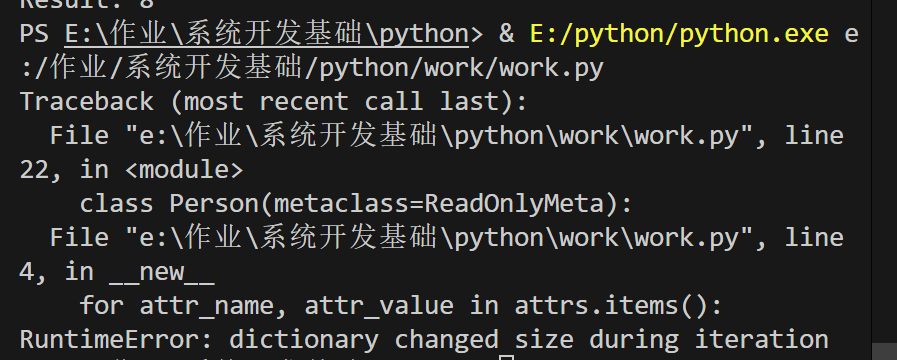
\includegraphics[width=\textwidth]{26} % 确保文件名正确
    \caption{效果展示}
  
  \end{figure}
\end{itemize}
\end{enumerate}






















%2.7LaTex=========================================================================%
\subsubsection{使用装饰器进行方法日志记录 }

\begin{enumerate}
  \item 创建一个装饰器,用于记录每次方法调用的日志。
  \begin{itemize}
  \item 命令展示
  \begin{verbatim}
def log_method_call(func):
    def wrapper(*args, **kwargs):
        print(f"Calling method: {func.__name__} with arguments: {args}, {kwargs}")
        result = func(*args, **kwargs)
        print(f"Method {func.__name__} returned: {result}")
        return result
    return wrapper

class Calculator:
    @log_method_call
    def add(self, a, b):
        return a + b

    @log_method_call
    def multiply(self, a, b):
        return a * b

# 使用示例
calc = Calculator()
result_add = calc.add(5, 3)       # 记录调用
result_multiply = calc.multiply(4, 2)  # 记录调用
 \end{verbatim}

  \item 效果展示
  \begin{figure}[H]
    \centering
    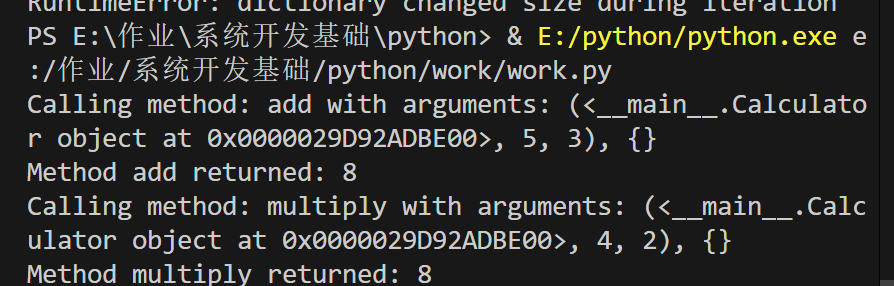
\includegraphics[width=\textwidth]{27} % 确保文件名正确
    \caption{效果展示}
  
  \end{figure}
\end{itemize}
\end{enumerate}































































  \subsection{大杂烩}
  {\color{blue}大杂烩展示}



%1.1LaTex=========================================================================%
%1.8LaTex=========================================================================%
\subsubsection{Markdown表格}

\begin{enumerate}
  \item Markdown支持使用管道符号(|)创建表格。表格可以非常方便地用于展示数据。


  \begin{itemize}
  \item 命令展示
  \begin{verbatim}

| 姓名   | 年龄 | 职业      |
|--------|------|-----------|
| Alice  | 30   | 软件工程师 |
| Bob    | 25   | 数据分析师 |
| Charlie| 35   | 产品经理   |





  \end{verbatim}
\item 效果展示
 
\begin{figure}[H]
    \centering
    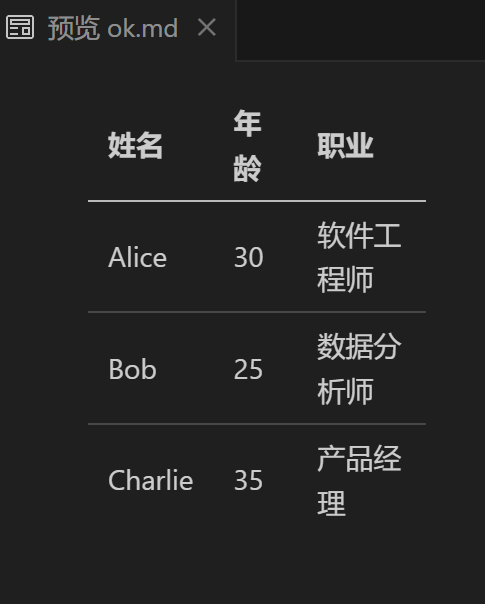
\includegraphics[width=\textwidth]{4.1} % 替换为您的图片文件名
    \caption{效果展示}
  \end{figure}
  \end{itemize}
\end{enumerate}

%1.9LaTex=========================================================================%
%1.8LaTex=========================================================================%
\subsubsection{Markdown嵌套列表}

\begin{enumerate}
  \item 子项目之前添加空格或制表符来实现。
  \begin{itemize}
  \item 命令展示
  \begin{verbatim}
1. 第一项
   - 子项 1
   - 子项 2
2. 第二项
   1. 子子项 1
   2. 子子项 2




  \end{verbatim}
\begin{figure}[H]
    \centering
    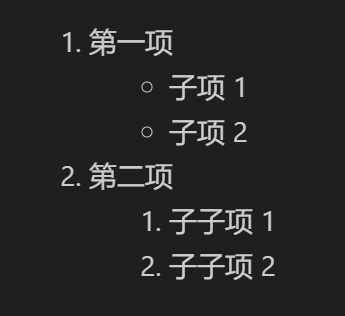
\includegraphics[width=\textwidth]{42} % 替换为您的图片文件名
    \caption{效果展示}
  \end{figure}
  \end{itemize}
\end{enumerate}

%1.9LaTex=========================================================================%
%1.8LaTex=========================================================================%
\subsubsection{引用块}

\begin{enumerate}
  \item 引用块可以用于引用其他人的话或文献,也可以嵌套使用
  \begin{itemize}
  \item 命令展示
  \begin{verbatim}

> 这是一个引用块。
> 
> > 这是一个嵌套引用块。


  \end{verbatim}
\item 效果展示
 \begin{figure}[H]
    \centering
    
\includegraphics[width=\textwidth]{43} % 替换为您的图片文件名
    \caption{效果展示}
  \end{figure}
  \end{itemize}
\end{enumerate}

%1.9LaTex=========================================================================%


%1.9LaTex=========================================================================%
\subsubsection{ 任务列表}

\begin{enumerate}
  \item 使用 - [ ] 和 - [x] 来表示未完成和已完成的任务。
  \begin{itemize}
  \item 命令展示
  \begin{verbatim}- [ ] 任务 1
- [x] 任务 2
- [ ] 任务 3







  \end{verbatim}

\item 效果展示
 \begin{figure}[H]
    \centering
    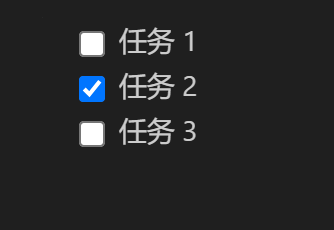
\includegraphics[width=\textwidth]{44} % 替换为您的图片文件名
    \caption{效果展示}
  \end{figure}
  \end{itemize}
\end{enumerate}


%1.2LaTex=========================================================================%
\subsubsection{自定义链接和图片}

\begin{enumerate}
  \item 可以使用方括号和圆括号来实现。
  \begin{itemize}
  \item 命令展示
  \begin{verbatim}
[GitHub](https://github.com) 是一个流行的代码托管平台。

![示例图片](https://via.placeholder.com/150 "示例图片")

  \end{verbatim}
\item 效果展示

 \begin{figure}[H]
   
    
\includegraphics[width=\textwidth]{45} % 替换为您的图片文件名
   
  \end{figure}

  \end{itemize}
\end{enumerate}























%1.3LaTex=========================================================================%
  \subsection{PyTorch编程}
  {\color{blue}PyTorch编程展示}






%3.1LaTex=========================================================================%
\subsubsection{自定义自动微分}

\begin{enumerate}
  \item 自动微分功能允许定义自定义的前向和反向传播逻辑。
  \begin{itemize}
  \item 命令展示
  \begin{verbatim}
import torch
from torch.autograd import Function

class MyReLU(Function):
    @staticmethod
    def forward(ctx, input):
        ctx.save_for_backward(input)
        return input.clamp(min=0)

    @staticmethod
    def backward(ctx, grad_output):
        input, = ctx.saved_tensors
        grad_input = grad_output.clone()
        grad_input[input < 0] = 0
        return grad_input

# 使用自定义ReLU
x = torch.tensor([-1.0, 2.0, 3.0], requires_grad=True)
relu = MyReLU.apply
y = relu(x)
y.sum().backward()
print(x.grad)  # Output: tensor([0., 1., 1.])


    
  \end{verbatim}

\item 效果展示
 \begin{figure}[H]
    \centering
    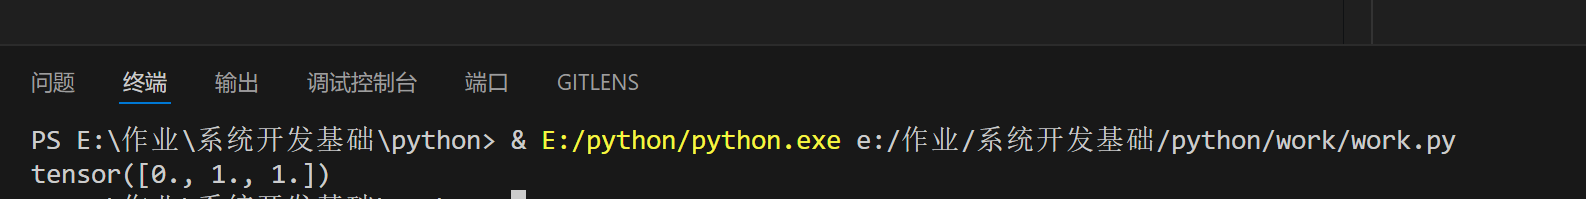
\includegraphics[width=\textwidth]{31} % 替换为您的图片文件名
    \caption{效果展示}
  \end{figure}

  \end{itemize}
\end{enumerate}















%3.2LaTex=========================================================================%
\subsubsection{动态计算图}

\begin{enumerate}
  \item PyTorch 的计算图是动态的,允许在每次迭代中更改模型的计算逻辑
  \begin{itemize}
  \item 命令展示
  \begin{verbatim}
 x = torch.tensor([1.0, 2.0, 3.0], requires_grad=True)
y = x * 2 if x.sum() > 0 else x / 2
y.sum().backward()
print(x.grad)  # Output: tensor([2., 2., 2.])


    
  \end{verbatim}

\item 效果展示
\item 效果展示
 \begin{figure}[H]
    \centering
    
\includegraphics[width=\textwidth]{32} % 替换为您的图片文件名
    \caption{效果展示}
  \end{figure}

  \end{itemize}
\end{enumerate}




















%3.3LaTex=========================================================================%
\subsubsection{自定义数据集}

\begin{enumerate}
  \item 使用 PyTorch 的 Dataset 和 DataLoader 来处理自定义数据
  \begin{itemize}
  \item 命令展示
  \begin{verbatim}
from torch.utils.data import Dataset, DataLoader

class MyDataset(Dataset):
    def __init__(self, data, labels):
        self.data = data
        self.labels = labels

    def __len__(self):
        return len(self.data)

    def __getitem__(self, idx):
        return self.data[idx], self.labels[idx]

data = torch.randn(100, 10)
labels = torch.randint(0, 2, (100,))
dataset = MyDataset(data, labels)
dataloader = DataLoader(dataset, batch_size=5, shuffle=True)
  \end{verbatim}
  
  \item 效果展示
  \begin{figure}[H]
    \centering
    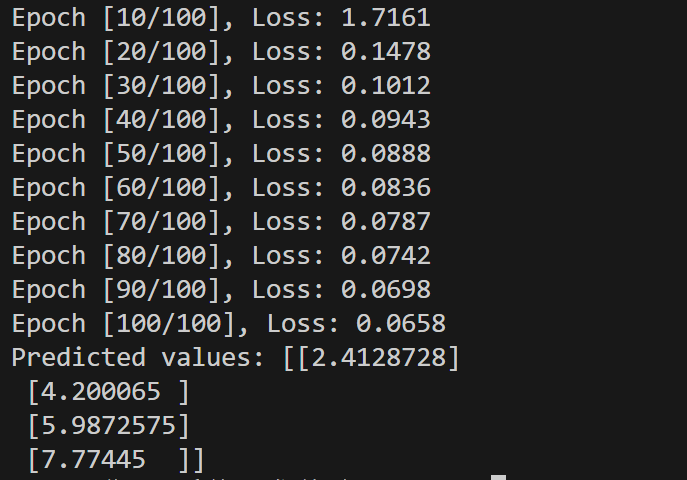
\includegraphics[width=\textwidth]{34} % 替换为您的图片文件名
    \caption{自定义数据集的示例} % 添加图片标题
  \end{figure}
  \end{itemize}
\end{enumerate}

























%3.4LaTex=========================================================================%
\subsubsection{线性回归}

\begin{enumerate}
  \item 线性回归分析
  \begin{itemize}
  \item 命令展示
  \begin{verbatim}
import torch
import torch.nn as nn
import torch.optim as optim

\# 定义简单的线性模型
class LinearRegressionModel(nn.Module):
    def __init__(self):
        super(LinearRegressionModel, self).__init__()
        self.linear = nn.Linear(1, 1)  \# 输入维度为1,输出维度为1

    def forward(self, x):
        return self.linear(x)

\# 准备数据
x_train = torch.tensor([[1.0], [2.0], [3.0], [4.0]], dtype=torch.float32)
y_train = torch.tensor([[2.0], [4.0], [6.0], [8.0]], dtype=torch.float32)

\# 实例化模型,定义损失函数和优化器
model = LinearRegressionModel()
criterion = nn.MSELoss()
optimizer = optim.SGD(model.parameters(), lr=0.01)

\# 训练模型
num_epochs = 100
for epoch in range(num_epochs):
    model.train()
    optimizer.zero_grad()
    outputs = model(x_train)
    loss = criterion(outputs, y_train)
    loss.backward()
    optimizer.step()

    if (epoch+1) % 10 == 0:
        print(f'Epoch [{epoch+1}/{num_epochs}], Loss: {loss.item():.4f}')

\# 测试模型
model.eval()
with torch.no_grad():
    predicted = model(x_train).numpy()
    print("Predicted values:", predicted)


    
  \end{verbatim}

 
\item 效果展示
  \begin{figure}[H]
    \centering
    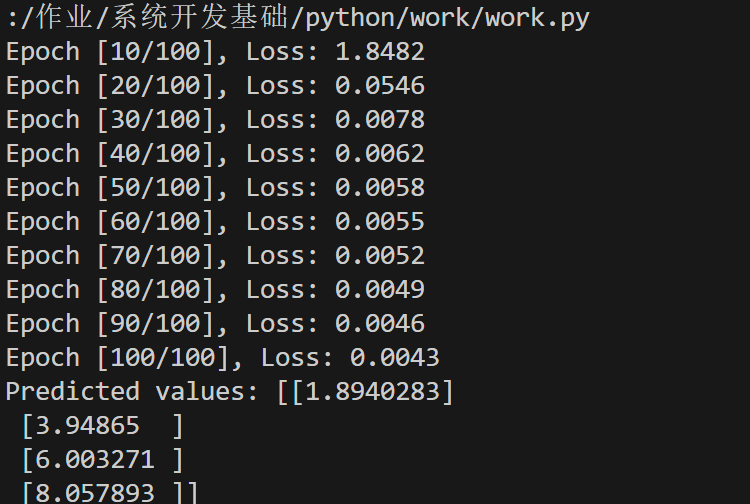
\includegraphics[width=\textwidth]{334} % 替换为您的图片文件名
    \caption{线性回归模型的预测结果} % 添加图片标题
  \end{figure}
  \end{itemize}
\end{enumerate}

















%3.5LaTex=========================================================================%
\subsubsection{神经网络分类器}

\begin{enumerate}
  \item 神经网络分类器
  \begin{itemize}
  \item 命令展示
  \begin{verbatim}
import torch
import torch.nn as nn
import torch.optim as optim

# 生成随机数据
def generate_data(num_samples=1000, num_features=20, num_classes=2):
    X = torch.randn(num_samples, num_features)  # 随机生成特征数据
    y = torch.randint(0, num_classes, (num_samples,))  # 随机生成0或1作为标签
    return X, y

# 定义简单的神经网络模型
class SimpleNN(nn.Module):
    def __init__(self, input_size, hidden_size, num_classes):
        super(SimpleNN, self).__init__()
        self.layer1 = nn.Linear(input_size, hidden_size)
        self.layer2 = nn.Linear(hidden_size, num_classes)
        self.relu = nn.ReLU()
        self.sigmoid = nn.Sigmoid()

    def forward(self, x):
        x = self.relu(self.layer1(x))
        x = self.layer2(x)
        return x

# 生成数据
X_train, y_train = generate_data()
X_test, y_test = generate_data()

# 转换为PyTorch张量
y_train = y_train.float().view(-1, 1)
y_test = y_test.float().view(-1, 1)

# 实例化模型,定义损失函数和优化器
input_size = X_train.shape[1]
hidden_size = 64
num_classes = 1  # 二分类任务
model = SimpleNN(input_size, hidden_size, num_classes)
criterion = nn.BCEWithLogitsLoss()  # 使用带有sigmoid激活的二元交叉熵损失
optimizer = optim.Adam(model.parameters(), lr=0.001)

# 训练模型
num_epochs = 100
for epoch in range(num_epochs):
    model.train()
    optimizer.zero_grad()
    outputs = model(X_train)
    loss = criterion(outputs, y_train)
    loss.backward()
    optimizer.step()

    if (epoch+1) % 10 == 0:
        print(f'Epoch [{epoch+1}/{num_epochs}], Loss: {loss.item():.4f}')

# 测试模型
model.eval()
with torch.no_grad():
    outputs = model(X_test)
    predicted = (outputs > 0).float()
    accuracy = (predicted.eq(y_test).sum() / y_test.shape[0]).item()
    print(f'Accuracy: {accuracy:.4f}')

  \end{verbatim}

\item 效果展示
  \begin{figure}[H]
    \centering
    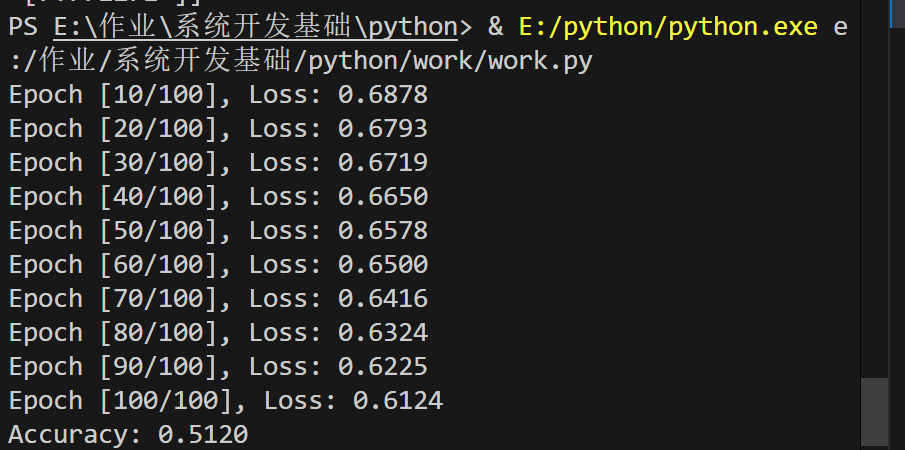
\includegraphics[width=\textwidth]{335} % 替换为您的图片文件名
    \caption{效果展示}
  \end{figure}
  \end{itemize}
\end{enumerate}





















%3.6LaTex=========================================================================%
\subsubsection{卷积神经网络(CNN)进行图像分类}

\begin{enumerate}
  \item 用 PyTorch 中的 CNN 来在随机生成的图像数据上进行分类。
  \begin{itemize}
  \item 命令展示
  \begin{verbatim}
import torch
import torch.nn as nn
import torch.optim as optim

# 定义简单的卷积神经网络
class SimpleCNN(nn.Module):
    def __init__(self):
        super(SimpleCNN, self).__init__()
        self.layer1 = nn.Conv2d(1, 16, kernel_size=3, stride=1, padding=1)
        self.layer2 = nn.Conv2d(16, 32, kernel_size=3, stride=1, padding=1)
        self.fc1 = nn.Linear(32*8*8, 128)
        self.fc2 = nn.Linear(128, 10)

    def forward(self, x):
        x = torch.relu(self.layer1(x))
        x = torch.max_pool2d(x, 2)
        x = torch.relu(self.layer2(x))
        x = torch.max_pool2d(x, 2)
        x = x.view(x.size(0), -1)
        x = torch.relu(self.fc1(x))
        x = self.fc2(x)
        return x

# 生成随机数据
def generate_image_data(num_samples=1000, image_size=(1, 32, 32), num_classes=10):
    X = torch.randn(num_samples, *image_size)
    y = torch.randint(0, num_classes, (num_samples,))
    return X, y

# 生成数据
X_train, y_train = generate_image_data()
X_test, y_test = generate_image_data()

# 实例化模型,定义损失函数和优化器
model = SimpleCNN()
criterion = nn.CrossEntropyLoss()
optimizer = optim.Adam(model.parameters(), lr=0.001)

# 训练模型
num_epochs = 10
batch_size = 64
for epoch in range(num_epochs):
    model.train()
    for i in range(0, len(X_train), batch_size):
        inputs = X_train[i:i + batch_size]
        targets = y_train[i:i + batch_size]

        optimizer.zero_grad()
        outputs = model(inputs)
        loss = criterion(outputs, targets)
        loss.backward()
        optimizer.step()

    print(f'Epoch [{epoch+1}/{num_epochs}], Loss: {loss.item():.4f}')

# 测试模型
model.eval()
with torch.no_grad():
    outputs = model(X_test)
    _, predicted = torch.max(outputs, 1)
    accuracy = (predicted == y_test).sum().item() / y_test.size(0)
    print(f'Accuracy: {accuracy:.4f}')

  \end{verbatim}

\item 效果展示
  \begin{figure}[H]
    \centering
    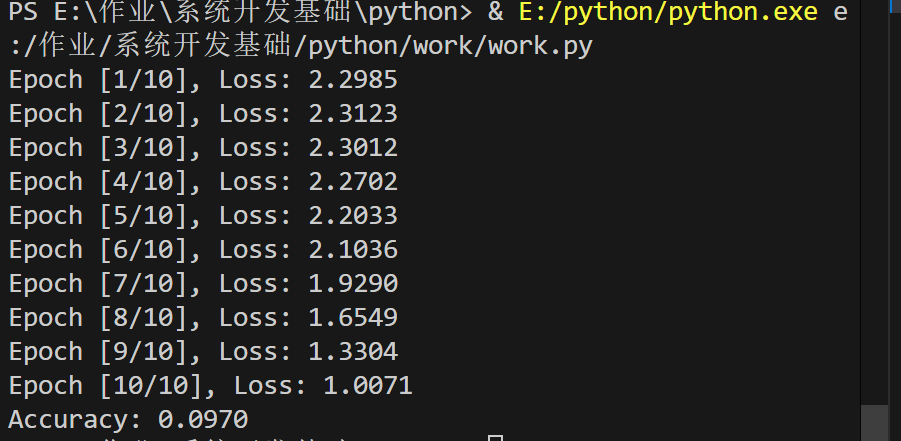
\includegraphics[width=\textwidth]{336} % 替换为您的图片文件名
    \caption{效果展示}
  \end{figure}
  \end{itemize}
\end{enumerate}




























%3.7LaTex=========================================================================%


\subsubsection{循环神经网络(RNN)进行序列预测}

\begin{enumerate}
  \item 使用 RNN 来模拟序列预测任务
  \begin{itemize}
  \item 命令展示
  \begin{verbatim}
import torch
import torch.nn as nn
import torch.optim as optim

# 生成随机数据
def generate_data(num_samples=1000, num_features=20, num_classes=2):
    X = torch.randn(num_samples, num_features)  # 随机生成特征数据
    y = torch.randint(0, num_classes, (num_samples,))  # 随机生成0或1作为标签
    return X, y

# 定义简单的神经网络模型
class SimpleNN(nn.Module):
    def __init__(self, input_size, hidden_size, num_classes):
        super(SimpleNN, self).__init__()
        self.layer1 = nn.Linear(input_size, hidden_size)
        self.layer2 = nn.Linear(hidden_size, num_classes)
        self.relu = nn.ReLU()
        self.sigmoid = nn.Sigmoid()

    def forward(self, x):
        x = self.relu(self.layer1(x))
        x = self.layer2(x)
        return x

# 生成数据
X_train, y_train = generate_data()
X_test, y_test = generate_data()

# 转换为PyTorch张量
y_train = y_train.float().view(-1, 1)
y_test = y_test.float().view(-1, 1)

# 实例化模型,定义损失函数和优化器
input_size = X_train.shape[1]
hidden_size = 64
num_classes = 1  # 二分类任务
model = SimpleNN(input_size, hidden_size, num_classes)
criterion = nn.BCEWithLogitsLoss()  # 使用带有sigmoid激活的二元交叉熵损失
optimizer = optim.Adam(model.parameters(), lr=0.001)

# 训练模型
num_epochs = 100
for epoch in range(num_epochs):
    model.train()
    optimizer.zero_grad()
    outputs = model(X_train)
    loss = criterion(outputs, y_train)
    loss.backward()
    optimizer.step()
import torch
import torch.nn as nn
import torch.optim as optim

# 定义简单的RNN模型
class SimpleRNN(nn.Module):
    def __init__(self, input_size, hidden_size, output_size):
        super(SimpleRNN, self).__init__()
        self.rnn = nn.RNN(input_size, hidden_size, batch_first=True)
        self.fc = nn.Linear(hidden_size, output_size)

    def forward(self, x):
        h0 = torch.zeros(1, x.size(0), hidden_size)
        out, _ = self.rnn(x, h0)
        out = self.fc(out[:, -1, :])
        return out

# 生成随机序列数据
def generate_sequence_data(num_samples=1000, seq_length=10, input_size=1, num_classes=2):
    X = torch.randn(num_samples, seq_length, input_size)
    y = torch.randint(0, num_classes, (num_samples,))
    return X, y

# 生成数据
input_size = 1
hidden_size = 16
output_size = 2
X_train, y_train = generate_sequence_data(num_samples=2000)
X_test, y_test = generate_sequence_data(num_samples=100)

# 实例化模型,定义损失函数和优化器
model = SimpleRNN(input_size, hidden_size, output_size)
criterion = nn.CrossEntropyLoss()
optimizer = optim.Adam(model.parameters(), lr=0.001)

# 训练模型
num_epochs = 10
batch_size = 64
for epoch in range(num_epochs):
    model.train()
    for i in range(0, len(X_train), batch_size):
        inputs = X_train[i:i + batch_size]
        targets = y_train[i:i + batch_size]

        optimizer.zero_grad()
        outputs = model(inputs)
        loss = criterion(outputs, targets)
        loss.backward()
        optimizer.step()

    print(f'Epoch [{epoch+1}/{num_epochs}], Loss: {loss.item():.4f}')

# 测试模型
model.eval()
with torch.no_grad():
    outputs = model(X_test)
    _, predicted = torch.max(outputs, 1)
    accuracy = (predicted == y_test).sum().item() / y_test.size(0)
    print(f'Accuracy: {accuracy:.4f}')

  \end{verbatim}

\item 效果展示
  \begin{figure}[H]
    \centering
    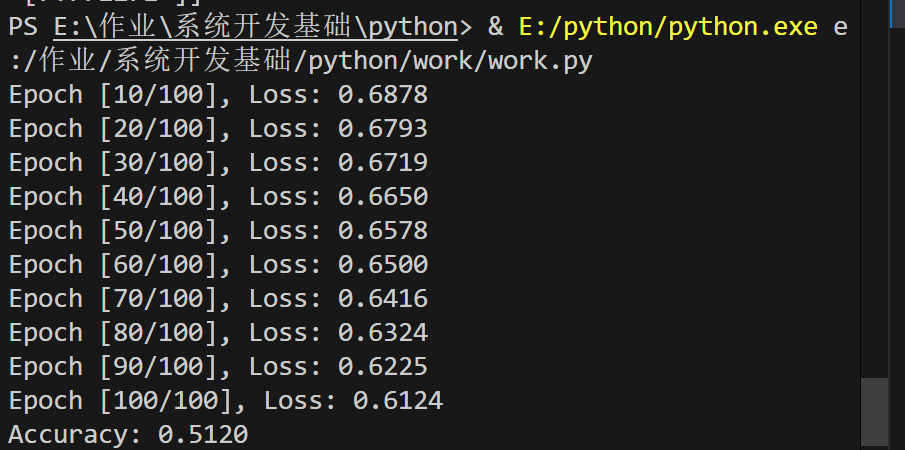
\includegraphics[width=\textwidth]{335} % 替换为您的图片文件名
    \caption{效果展示}
  \end{figure}
  \end{itemize}
\end{enumerate}























%3.8LaTex=========================================================================%

\subsubsection{自定义数据集和数据加载器}

\begin{enumerate}
  \item 使用 PyTorch 的 Dataset 和 DataLoader 来处理自定义数据。


  \begin{itemize}
  \item 命令展示
  \begin{verbatim}
import torch
from torch.utils.data import Dataset, DataLoader
import torch.nn as nn
import torch.optim as optim

# 自定义数据集
class MyDataset(Dataset):
    def __init__(self, num_samples=1000, num_features=10):
        self.data = torch.randn(num_samples, num_features)
        self.labels = (self.data.sum(axis=1) > 0).float()

    def __len__(self):
        return len(self.data)

    def __getitem__(self, idx):
        return self.data[idx], self.labels[idx]

# 定义简单的神经网络模型
class SimpleNN(nn.Module):
    def __init__(self, input_size):
        super(SimpleNN, self).__init__()
        self.layer1 = nn.Linear(input_size, 64)
        self.layer2 = nn.Linear(64, 1)

    def forward(self, x):
        x = torch.relu(self.layer1(x))
        x = torch.sigmoid(self.layer2(x))
        return x

# 实例化数据集和数据加载器
dataset = MyDataset()
dataloader = DataLoader(dataset, batch_size=32, shuffle=True)

# 实例化模型,定义损失函数和优化器
input_size = dataset.data.shape[1]
model = SimpleNN(input_size)
criterion = nn.BCELoss()
optimizer = optim.Adam(model.parameters(), lr=0.001)

# 训练模型
num_epochs = 10
for epoch in range(num_epochs):
    model.train()
    for inputs, targets in dataloader:
        optimizer.zero_grad()
        outputs = model(inputs)
        loss = criterion(outputs, targets.unsqueeze(1))
        loss.backward()
        optimizer.step()

    print(f'Epoch [{epoch+1}/{num_epochs}], Loss: {loss.item():.4f}')

# 在训练数据上测试模型
model.eval()
with torch.no_grad():
    correct = 0
    total = 0
    for inputs, targets in dataloader:
        outputs = model(inputs)
        predicted = (outputs > 0.5).float()
        total += targets.size(0)
        correct += (predicted.squeeze(1) == targets).sum().item()
    accuracy = correct / total
    print(f'Accuracy: {accuracy:.4f}')

  \end{verbatim}
\item 效果展示
  \begin{figure}[H]
    \centering
    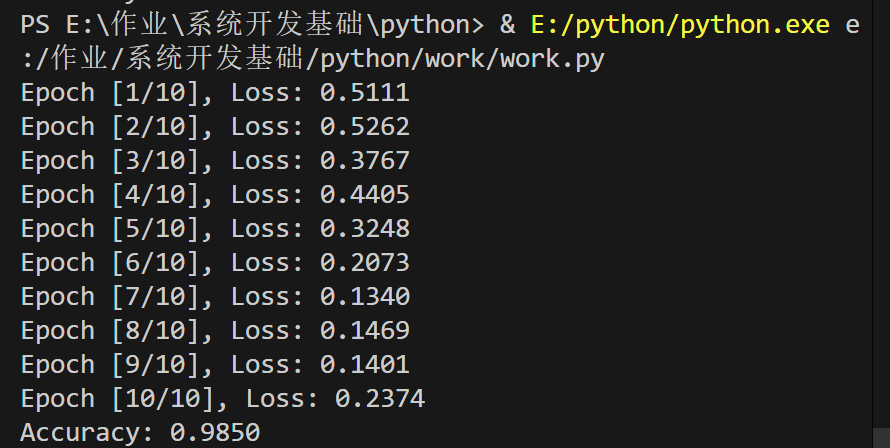
\includegraphics[width=\textwidth]{338} % 替换为您的图片文件名
    \caption{效果展示}
  \end{figure}
  \end{itemize}
\end{enumerate}

























%3.9LaTex=========================================================================%




















%3.10LaTex=========================================================================%

















%1.2.16表格==================================================%
 \section{困难与解决方案}
 \subsection{调试及性能分析}

\begin{enumerate}
 \item \begin{itemize}
 \item 问题:rr 的使用不成功,报告一个致命错误,指出它无法识别 Intel CPU 的微架构(Intel CPU type 0xb06a0 unknown)
 \item 解决方案:rr 不支持当前机器的 CPU 类型,或者 rr 版本过旧,未包括对新 CPU 的支持。从GitHub上下载最新的rr,来更新 rr。
 \end{itemize}

\item \begin{itemize}
 \item 问题:编译 rr 时遇到了与 32 位交叉编译相关的错误。
 \item 解决方案:安装 32 位库
 \end{itemize} 

\item \begin{itemize} 
\item 问题:下载pycallgraph库报错 
 \item 解决方案:pycallgraph 似乎不再维护,并且与较新的 Python 版本不兼容。由于该库依赖于较旧的工具和配置选项(例如 use2to3),这些选项在当前的 Python 和 setuptools 环境中不再支持,因此安装失败。所以换成其他的。
 \end{itemize} 
\item \begin{itemize}
 \item 问题:在使用journalctl命令时,未能成功获取到超级用户的日志信息。
\item 解决方案:使用sudo来提升权限,并正确指定用户ID(UID)过滤参数。
 \end{itemize}\item \begin{itemize}
\item 问题:在使用htop命令时,未能成功安装或启动。
\item 解决方案:确保系统已更新,并且正确安装了htop包,使用sudo apt-get install htop进行安装。
\end{itemize} \end{enumerate}




%1.2.16表格===========
\subsection{元编程演示}
 \begin{enumerate} 
\item 
\begin{itemize} 
\item 问题:make无法找到生成paper.pdf所需的paper.tex文件
\item 解决方案:确保所有在Makefile中列出的依赖文件都存在于当前目录中,同时检查和创建必要文件。
 \end{itemize} 
\item \begin{itemize}
\item 问题:在使用装饰器进行方法计时时,遇到了计时不准确的问题。
\item 解决方案:检查并确保在装饰器中正确地计算了时间差,并且没有其他代码干扰了计时。
\end{itemize}
\item \begin{itemize}
\item 问题:在使用元类创建只读属性时,未能正确限制属性的修改。
\item 解决方案:确保在元类中正确地定义了属性的getter和setter,并且setter抛出了适当的异常。
\end{itemize}
\end{enumerate}





%1.2.16表格===========
\subsection{PyTorch编程}

\begin{enumerate} 
\item \begin{itemize}
\item 问题:在自定义数据集时,遇到了数据加载不正确的问题。
\item 解决方案:检查数据集类的getitem方法,确保它正确地返回了数据和标签。
\end{itemize}
\item \begin{itemize}
\item 问题:在训练神经网络分类器时,模型的准确率未达到预期。
\item 解决方案:调整模型结构和参数,使用交叉验证来优化模型性能,并确保数据预处理正确。
\end{itemize}
\item \begin{itemize}
\item 问题:在实现卷积神经网络(CNN)时,遇到了模型不收敛的问题。
\item 解决方案:调整学习率和优化器参数,增加数据增强,以及使用合适的初始化方法。
\end{itemize}
 \end{enumerate}

%1.2.16表格==================================================% 
\section{心得体会}
 \begin{itemize} 
\item 通过本次的学习,我对调试工具和性能分析有了更深入的认识,学会了在Linux上使用journalctl来获取系统日志,使用stress和htop工具来模拟和监控系统负载。此外,我也掌握了如何使用linter插件来提高代码质量,以及如何通过netstat和lsof命令来查找并处理端口占用问题。 
\item 在元编程方面,我学习了如何使用装饰器和元类来增强代码的灵活性和可维护性,这些技术让我能够编写更加动态和强大的Python程序。
\item 通过PyTorch编程的学习,我对深度学习有了更实际的理解,特别是在图像处理和分类任务中。我学会了如何构建和训练神经网络,以及如何使用PyTorch提供的各种工具和类来处理数据和构建模型。
\item Markdown是非常有用的工具,通过本次学习我也学会了用Markdown绘制表格等功能,深刻了感受了Markdown的魅力。
\item 我期待将这些新学到的知识应用到未来的项目中,以解决更复杂的问题
\end{itemize}



  %1.2.16表格==================================================%

  \section{github网址}
\href{https://github.com/KeepingMoving/work1.git}{GitHub仓库}
https://github.com/KeepingMoving/work1.git
 










\end{document}
